\subsection{Rappel de la mission et des livrables}

Le projet \emph{bouclage de production} avait pour objectif de créer une solution universelle de gestion de la chaîne de production des \tgv pour tous les axes de la \sncf.

L'axe sud-est a développé sa propre solution avec des tableurs Excel, et des macros pour les remplir et les mettre à jour. Cette solution permettra aux équipes de \tnp d'avoir point de comparaison lors du développement.

\begin{figure}[H]
    \centering
    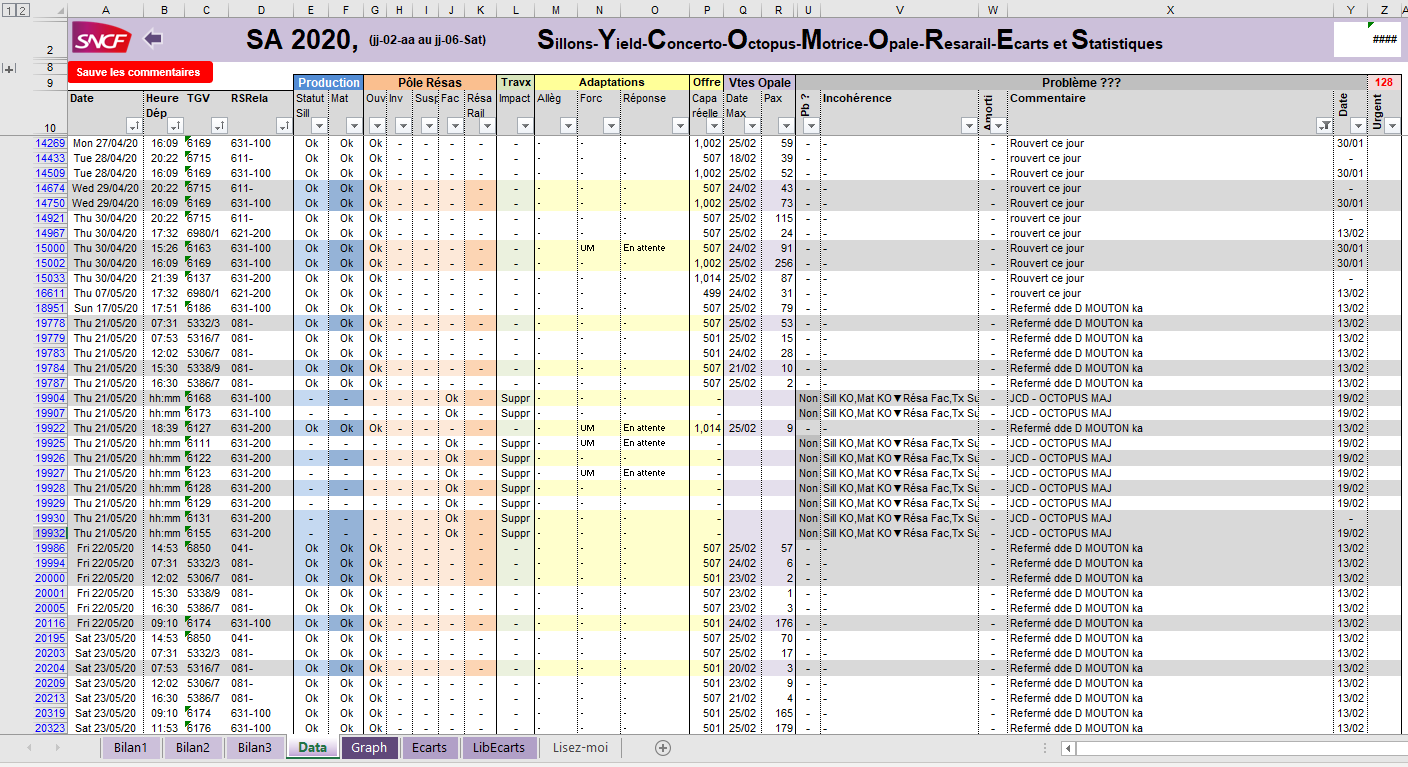
\includegraphics[width=1\linewidth]{img/data_bdp_sycomores.png}
    \caption{Fichier Excel utilisé par l'axe sud-est pour effectuer son bouclage de production}
\end{figure}

\damien a proposé à la \sncf un projet découpé en plusieurs lots, pour d'abord valider la faisabilité d'une solution puis d'avancer vers une industrialisation de celle-ci. Pour ce faire, \tnp fournira un \gls{poc} dans un premier temps, puis un \gls{mvp} avant de finir sur une solution finale robuste et pérenne.

  \begin{figure}[H]
    \centering
    
\includegraphics[width=0.8\linewidth]{img/planning-juillet-octobre-2019.png}
    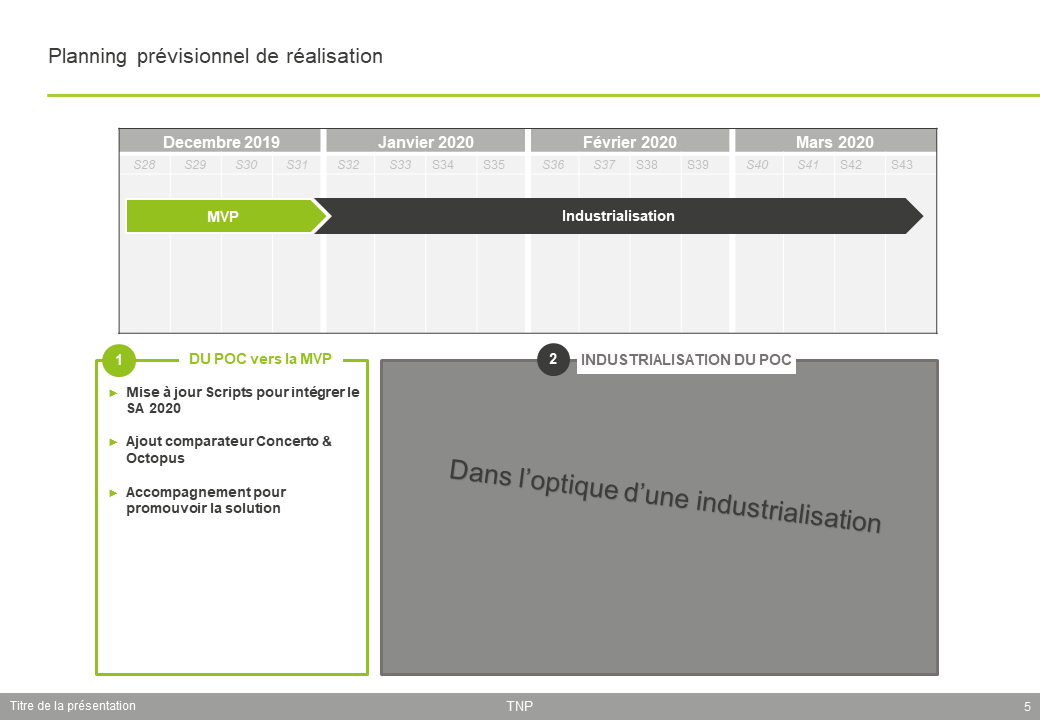
\includegraphics[width=0.8\linewidth]{img/planning-decembre-mars-2020-MVP.png}
    \caption{Les plannings du projet de juillet 2019 à mars 2020}
  \end{figure}

\newpage
\subsection{L'interface web}

\stefan et Adrien \textsc{Lemoine} -- les \gls{ux} -- ont travaillé sur les maquettes de l'interface web. Nous nous sommes basés sur celles-ci pour notre travail, ainsi que sur les fonctionnalités discutées en réunion de préparation de \textit{sprint}.

  \begin{figure}[H]
    \centering
    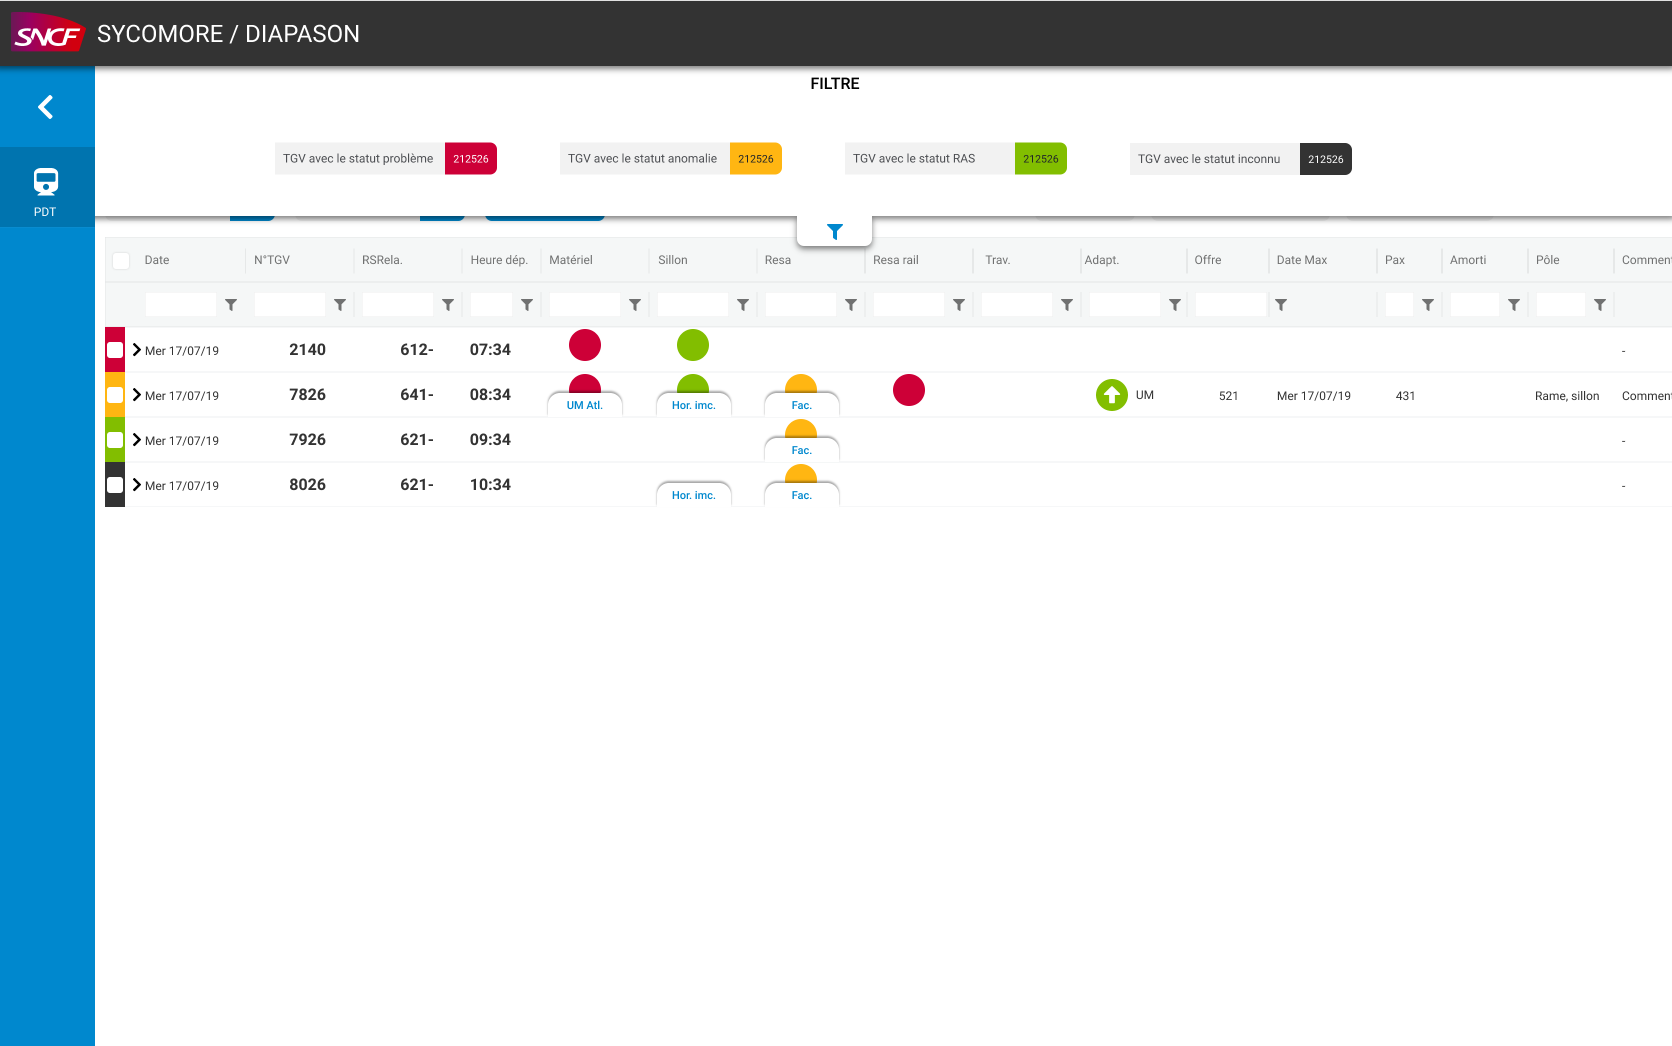
\includegraphics[width=0.58\linewidth]{img/maquette_home_page_filters.png}
    
\includegraphics[width=0.40\linewidth]{img/maquette_commentaire.png}
    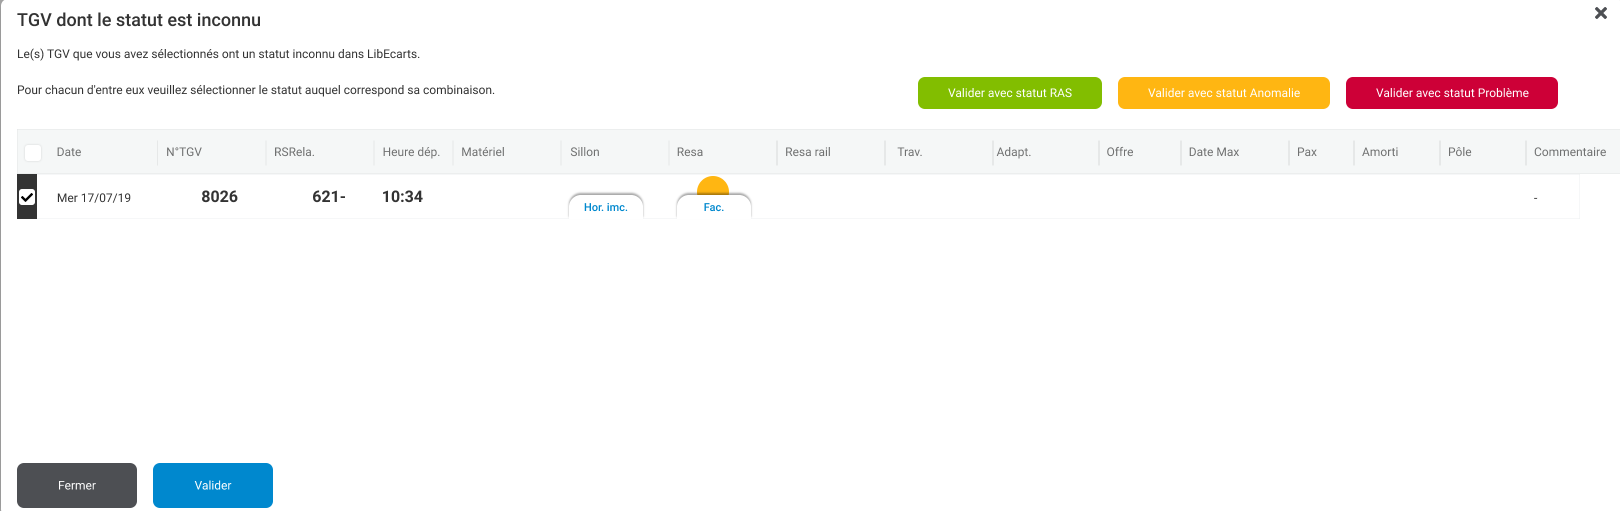
\includegraphics[width=1\linewidth]{img/maquette_create_libecart.png}
    \caption{Écrans principaux de la maquette : vue synthétique, filtres, ajout de commentaire et gestion des règles lib-écarts}
  \end{figure}

Nous nous sommes dirigés naturellement vers une interface web plutôt qu'une interface plus lourde, comme un logiciel par exemple. Tout d'abord parce que les salariés sont maintenant habitués à avoir leurs applicatifs et intranets sur leur navigateur Internet, et d'autre part parce que le web est peu gourmand, accessible partout et sur n'importe quel appareil. La solution sera donc encore plus accessible que le fichier Excel utilisé.

Comme choix de technologie web, nous aurions tout à fait pu utiliser le HTML/CSS classique, qui aurait parfaitement fonctionné. Cependant, nous disposions d'un délai de conception court et l'équipe de développeur était essentiellement composée de stagiaires et alternants, encore débutants dans le domaine. L'utilisation d'un 
\gls{framework}\footnote{\glsdesc{framework}.}
web a donc été privilégiée.

En effet, un \gls{framework} intègre souvent les éléments basiques dont on a besoin à chaque projet web, comme par exemple les fonctionnalités de communication avec un \gls{back-end} pour récupérer ou envoyer des données.

Ils permettent également d'utiliser des \og composants \fg web, qui ne sont rien d'autre que des morceaux indépendants d'interface que l'on peut insérer dans nos propres interfaces. Grâce à ce principe, les développeurs peuvent se concentrer sur les réelles fonctionnalités du principe en réutilisant des composants basiques comme des tableaux avec filtres. Pourquoi perdre du temps à inventer ce qui existe déjà ?

Il existe plusieurs \gls{framework} web sur le marché, les plus connus étant VueJS\cite{noauthor_vuejs_nodate}, ReactJS\cite{noauthor_react_nodate} et Angular\cite{noauthor_angular_nodate}. C'est ce dernier que nous avons gardé. J'avais déjà travaillé un an avec Angular au cours de ma première année d'alternance, lorsque j'étais chez Milleis Banque avec \damien. J'étais donc déjà à l'aise avec cette technologie, ce qui nous évitait un temps d'adaptation et d'apprentissage.

De plus, c'est le \gls{framework} le plus complet des 3. Si bien que l'on peut créer une application web sans sortir d'Angular, tandis que ReactJS et VueJS nécessitent l'utilisation de bibliothèques externes. Ils se reposent sur le travail déjà existant de la communauté web. Ils sont dans ce sens meilleures si l'on souhaite se créer des connaissances plus complètes dans le domaine du développement \gls{front-end}, mais prennent de ce fait plus de temps à prendre en main. Comme nous n'avions pas d'expert dans l'équipe, il était plus simple de se réfugier dans le confort que propose Angular.

Une fois la technologie de développement web choisie, il nous restait à trouver les composants web qui allaient nous permettre de gagner du temps sur la conception des interfaces pour nous concentrer sur les vraies fonctionnalités du projet.
Le plus gros de l'interface est le tableau présentant les données synthétiques et permettant l'utilisation de nombreux filtres et tris. En effet, le but était de présenter les données de la manière la plus efficace possible, et de permettre une recherche de la donnée rapide. Comme ce que l'on retrouve sur un fichier Excel.

\damien avait déjà regardé en amont s'il existait ce type de composants. Le fait d'avoir le plus gros de l'interface déjà créé par la communauté web permet de réduire considérablement le temps passé sur les tâches, et impacte donc nécessairement le planning présenté au client.

Il avait trouvé le composant web \textit{AgGrid}\cite{noauthor_ag-grid_nodate-1}, qui répondait parfaitement à nos besoins. Il s'agit d'un tableau intégrant des fonctions de tri et de recherche par défaut, et proposant même un chargement dynamique des données.


  \begin{figure}[H]
    \centering
    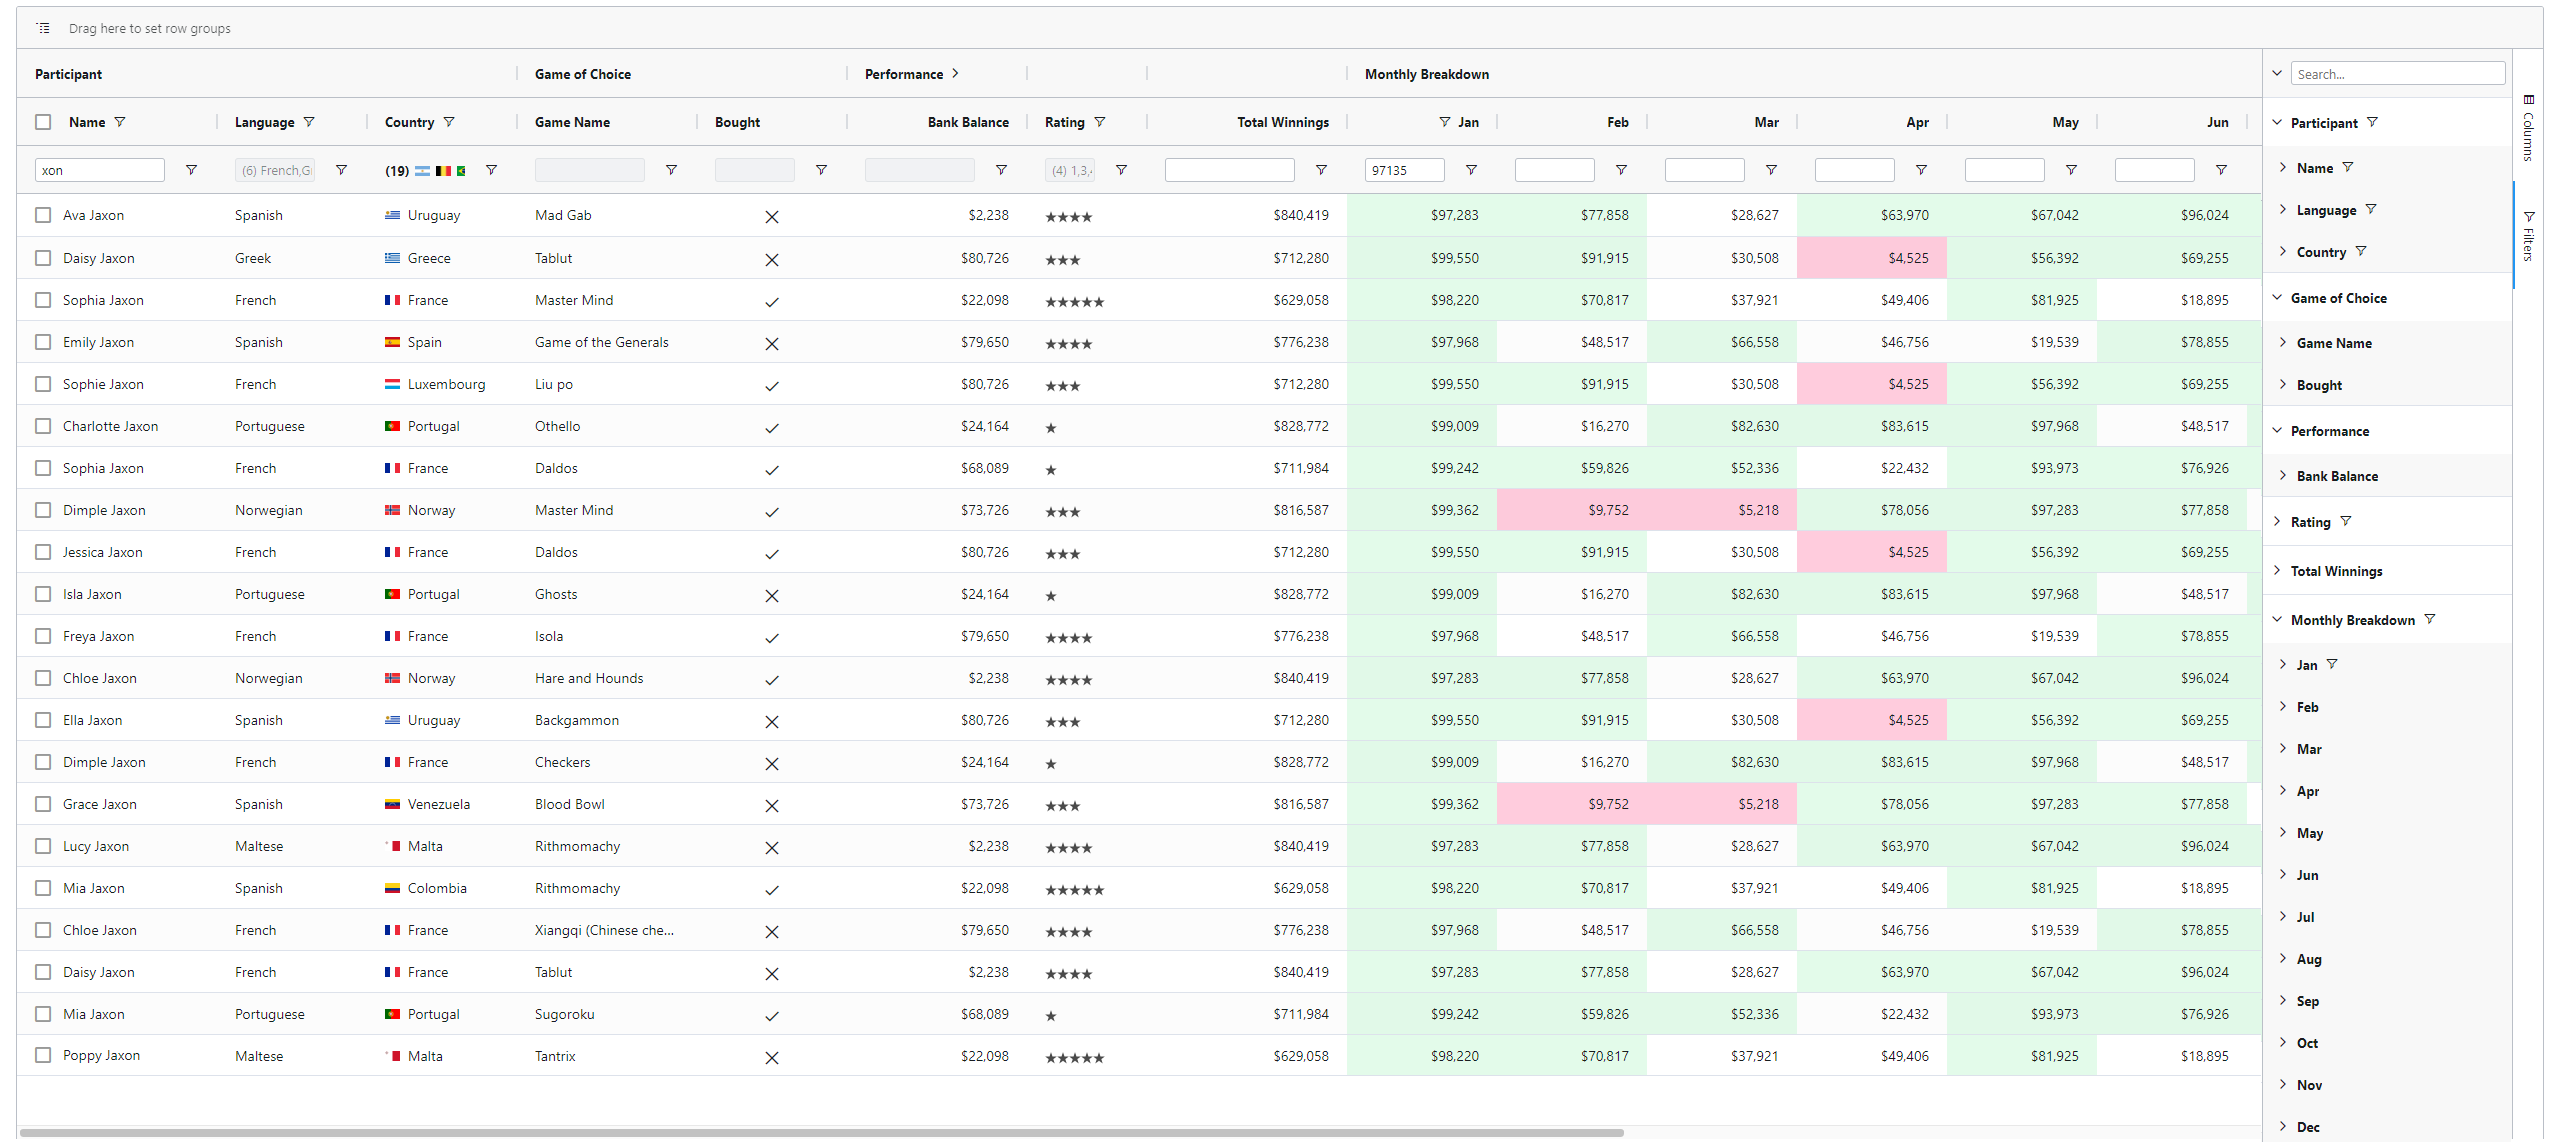
\includegraphics[width=1\linewidth]{img/ag-grid-demo.png}
    \caption{Page de démonstration du composant \textit{AgGrid}\cite{noauthor_demo_nodate}}
  \end{figure}

Cette dernière fonctionnalité était importante à prendre en compte, puisque même si de prime abord elle ne faisait pas partie du besoin du client -- qui se limitait à une recherche et des tris --, elle a un grand impact à l'usage de l'application.

En effet, le volume de données présenté dans la vue est considérable. La base contient plus de 100 000 informations de trains au total, et même une fois les filtres de base appliqués -- nous ne montrons à l'utilisateur que les trains concernant son axe, et la période dans laquelle il se trouve --, le volume total atteint tout de même plus de 25 000 trains.

Charger les données de 25 000 trains à chaque ouverture de l'application serait beaucoup trop long, et pas utilisable au quotidien. Il fallait donc absolument une solution nous permettant de charger les données uniquement lorsque c'était nécessaire.

Je me suis d'abord occupé de la partie \og chargement des données \fg de AgGrid. Pour ce faire, j'ai suivi la documentation d'AgGrid, et notamment la partie 
\textit{Server-Side Row Model}\cite{noauthor_server-side_nodate}
qui étend la fonctionnalité d'
\textit{Infinite Row Model}\cite{noauthor_ag-grid_nodate}.

L'
\textit{Infinite Row Model}
permet charger les données au fur et à mesure que l'utilisateur fait défiler les données dans le tableau. Cela est rendu possible en développant nous-mêmes la fonction de récupération de données par blocs côté serveur. On n'envoie plus toutes les données en une seule fois, mais on envoie des blocs de données.

  \begin{figure}[H]
    \centering
    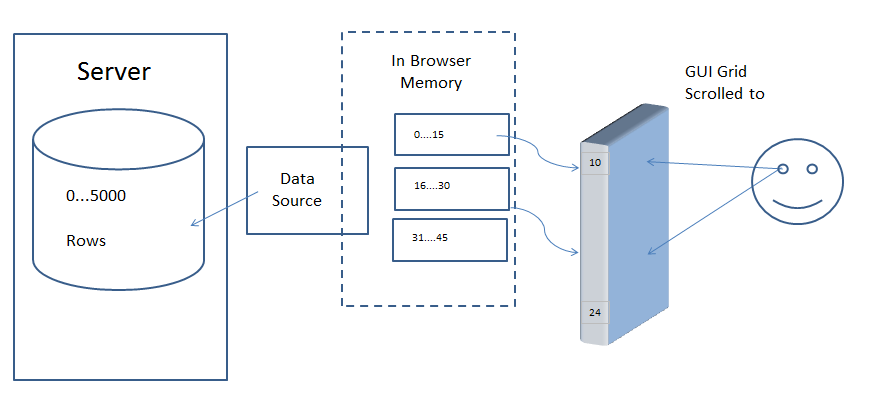
\includegraphics[width=1\linewidth]{img/high-level.png}
    \caption{
L'\textit{Infinite Row Model}, permettant de charger les données au fur et à mesure, bloc par bloc.
    }
  \end{figure}
  
Par exemple, au premier chargement, l'interface demandera au serveur les trains de l'index 1 à 500. Quand l'utilisateur fera défiler le tableau, elle demandera alors les trains de l'index 500 à 1000, et ce ainsi de suite jusqu'à tout afficher.

A cela vient s'ajouter le
\textit{Server-Side Row Model}
, permettant d'ajouter les fonctions de tris et de filtres aux données récupérées.
\textit{AgGrid} gère normalement de base ces fonctions, comme on l'a vu dans sa présentation. Cependant, dans un contexte de chargement des données côté serveur, il lui est impossible d'utiliser ses propres fonctions de tris et de filtres.

  \begin{figure}[H]
    \centering
    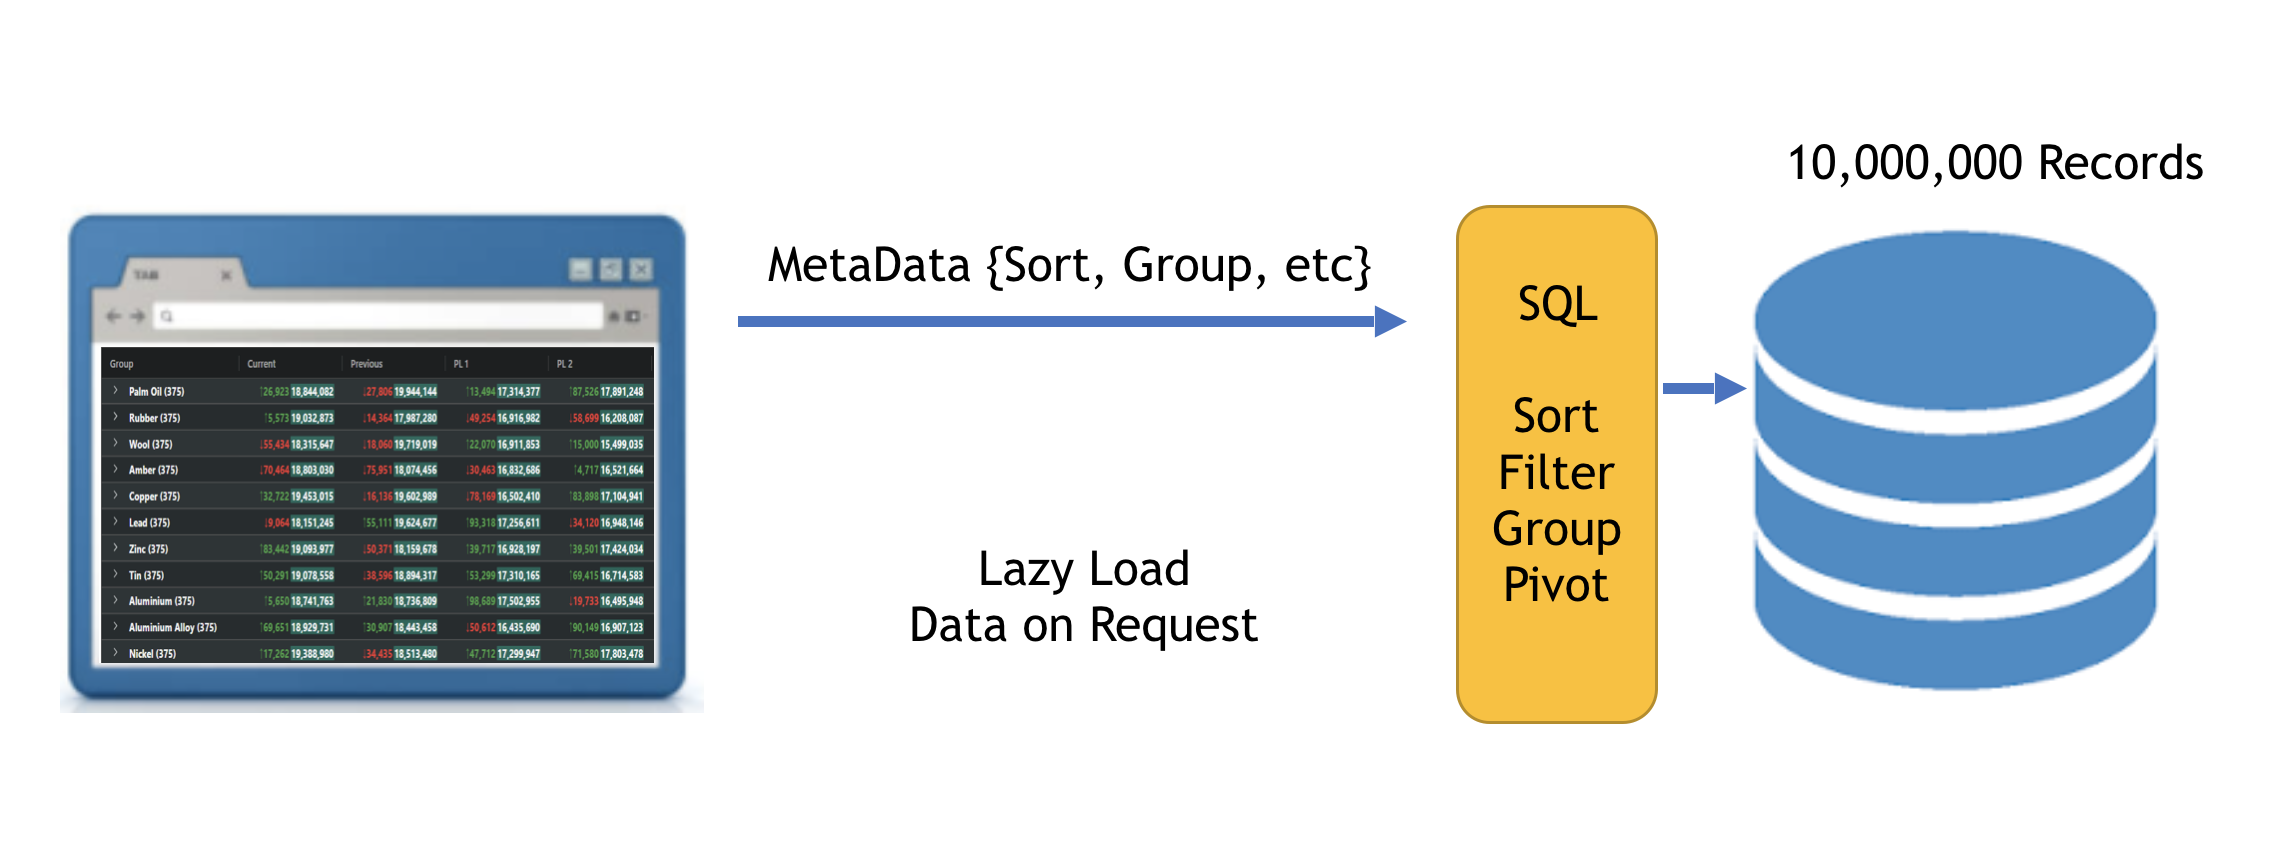
\includegraphics[width=1\linewidth]{img/enterprise-row-model.png}
    \caption{
Le \textit{Server-Side Row Model} permet de garder les fonctionnalités de filtres et de tris lorsque l'on utilise l'\textit{Infinite Row Model}
    }
  \end{figure}
  
En effet, le tableau n'a plus accès à la totalité des données puisqu'elles sont chargées au fur et à mesure. Comment pourrait-il effectuer une recherche s'il n'a pas toutes les données ? Nous avons donc développé toutes ces fonctions côté serveur avec Anthony \textsc{Mercadal}, mon collègue développeur \gls{full-stack}.


  \begin{figure}[H]
    \centering
    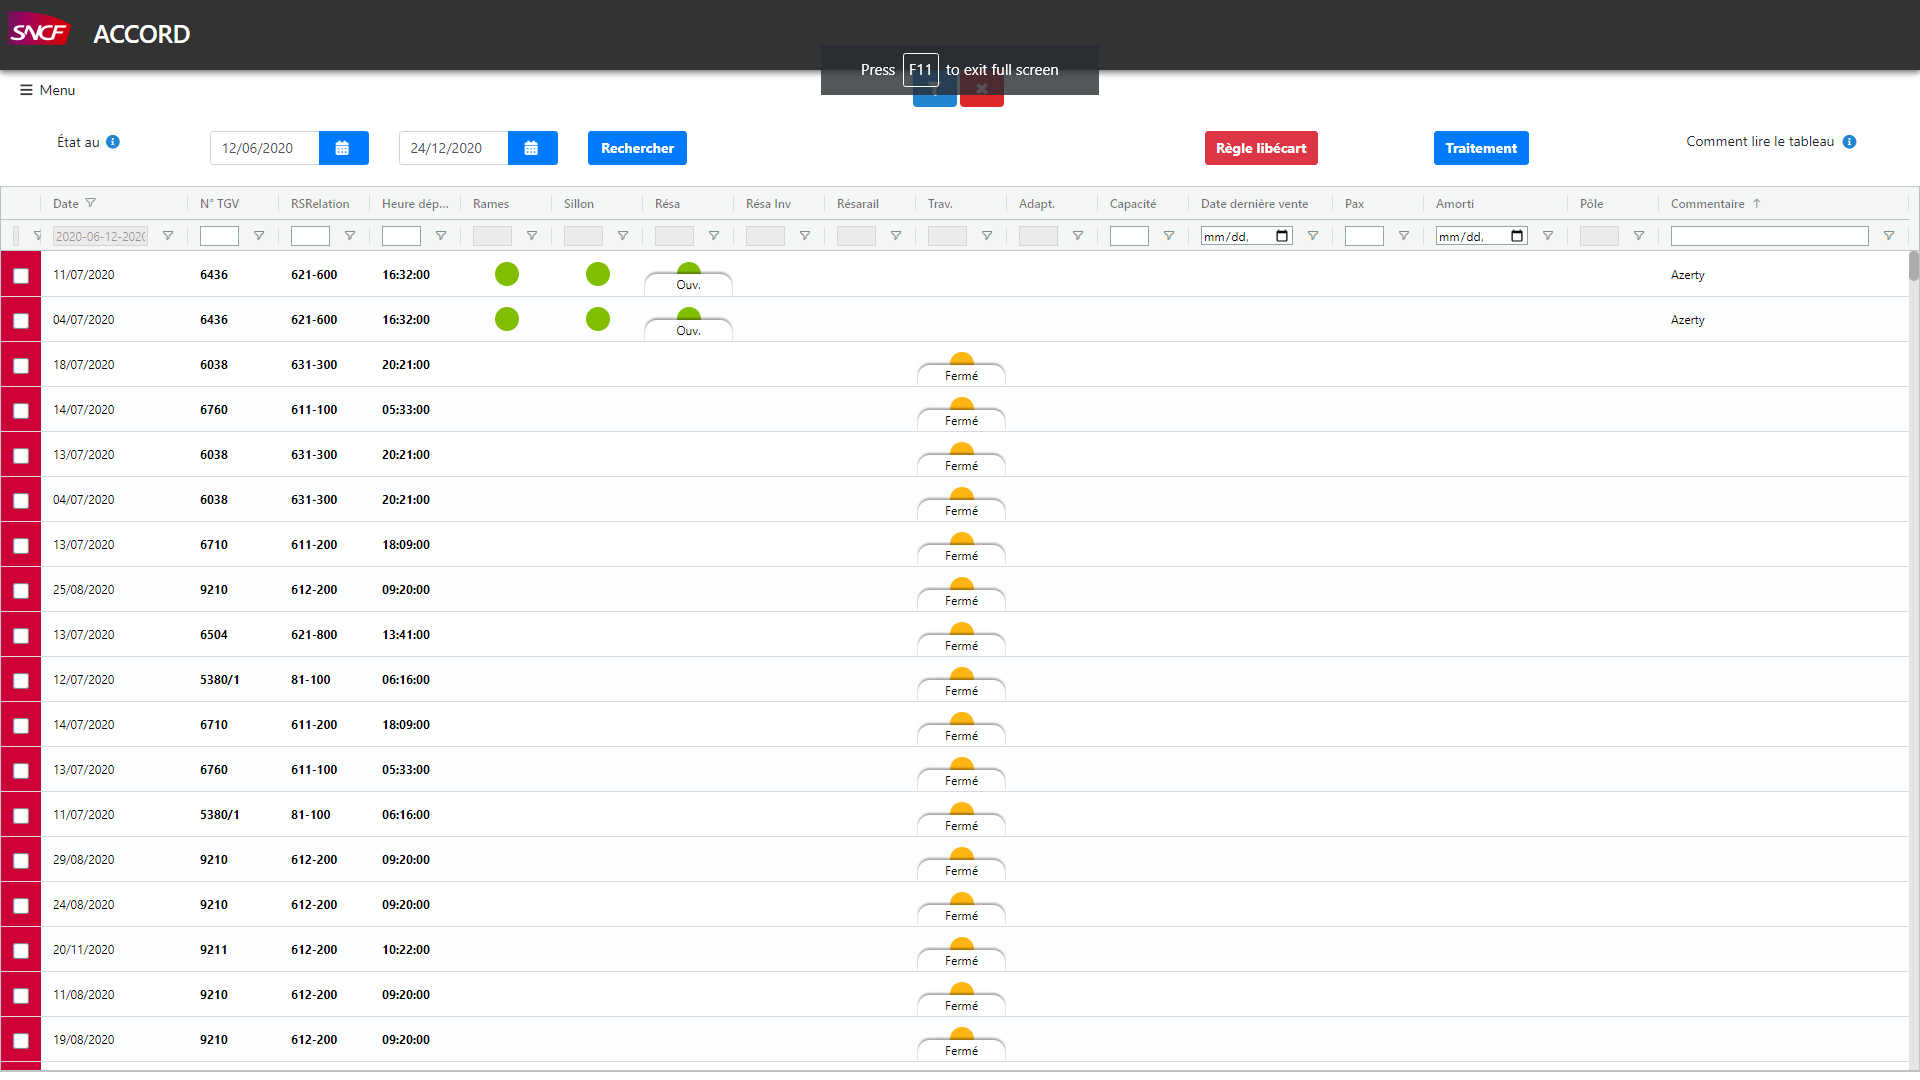
\includegraphics[width=1\linewidth]{img/sycomores_home.png}
    \caption{Tableau de synthèse du bouclage de production, avec fonctions de tris et de filtres sur ses colonnes}
  \end{figure}

Une fois cette partie terminée, j'ai travaillé sur la page de gestion des règles lib-écarts. Encore une fois, dans une optique de ne pas perdre de temps à recréer ce qui existe déjà nous avons fait le choix d'utiliser 
\textit{Bootstrap}\cite{noauthor_bootstrap_nodate}.
Il s'agit d'une bibliothèque contenant tous les éléments de base d'une interface web déjà stylisés. En plus de ces éléments, la grande force de cette bibliothèque est leur système de grille permettant de positionner très facilement les éléments dans l'interface.

  \begin{figure}[H]
    \centering
    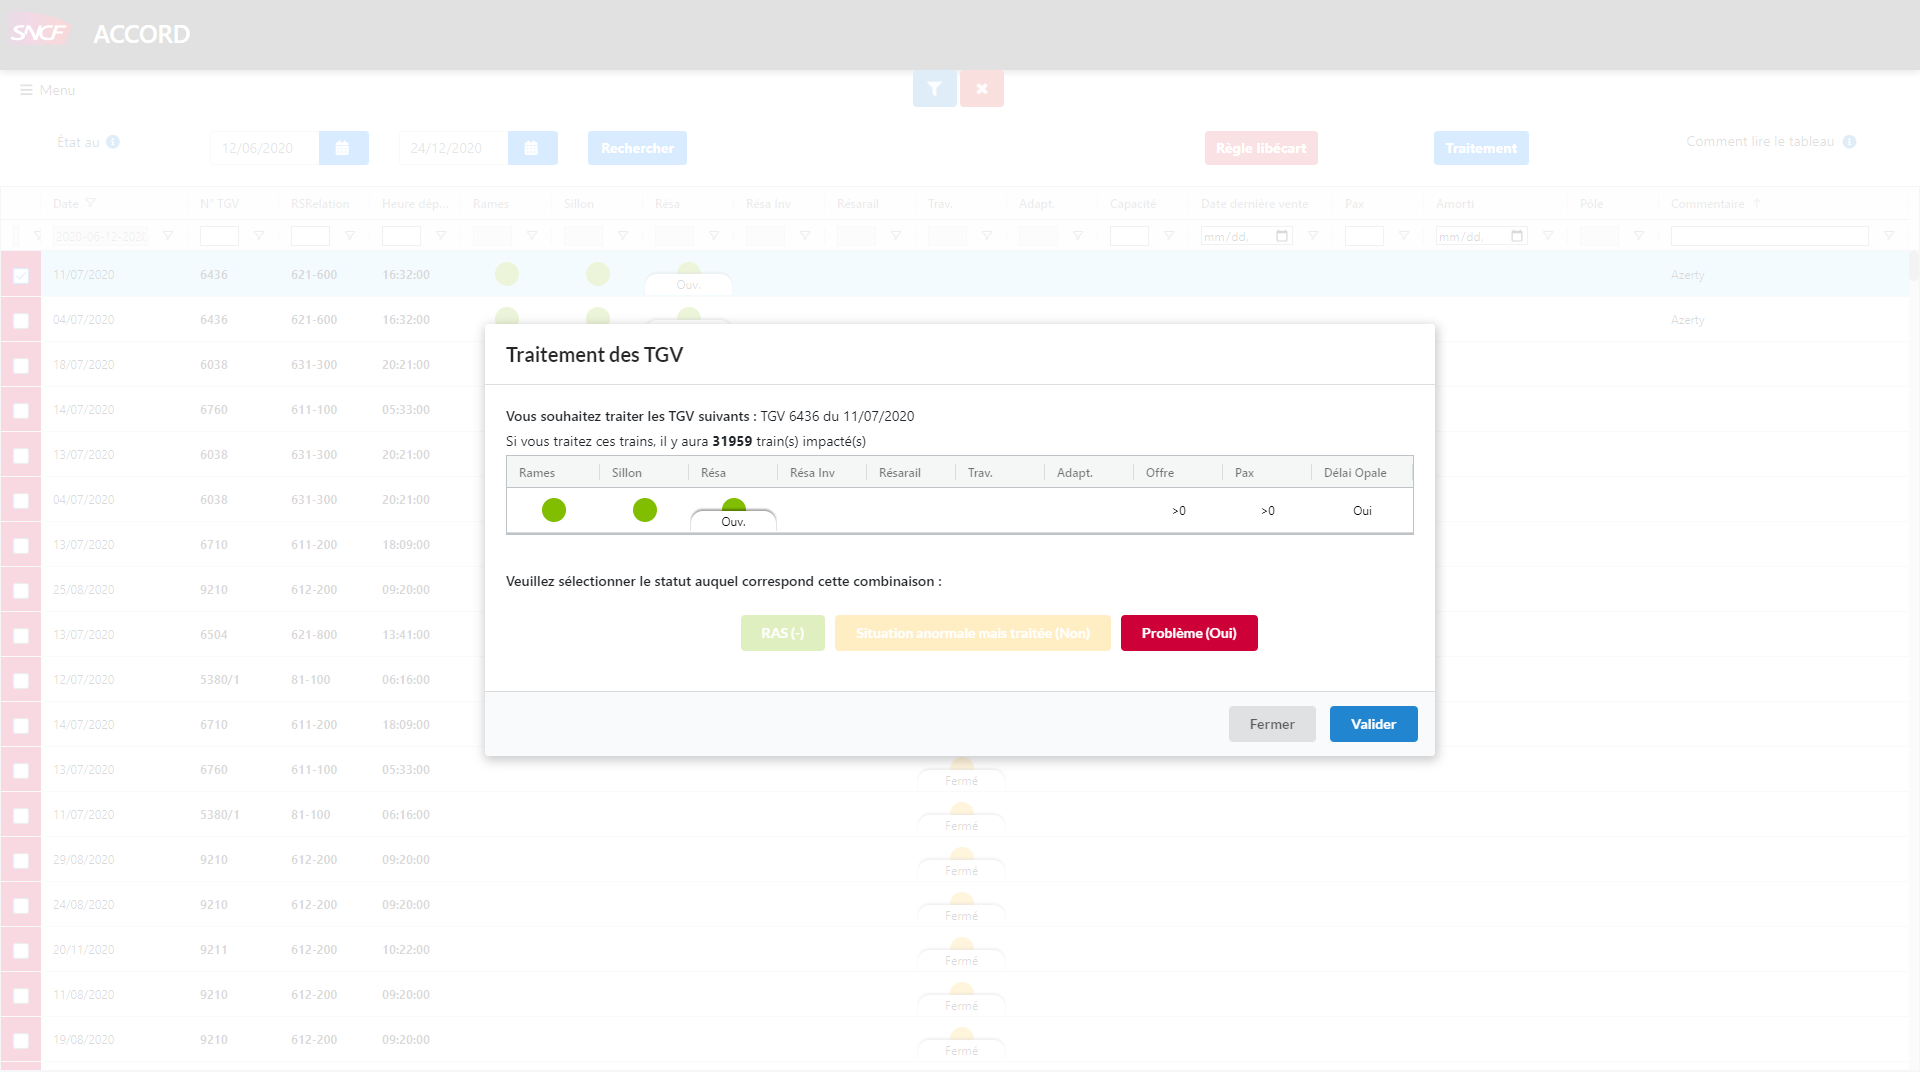
\includegraphics[width=1\linewidth]{img/sycomores_regle_libecart.png}
    \caption{Page de gestion des règles lib-écarts}
  \end{figure}

Cette page permet de modifier ou créer une règle lib-écart. Ainsi, tous les trains ayant les mêmes statuts dans les différentes sources se verront assigner le même statut lib-écart que nous avions vu dans la partie \og découpage de la mission \fg.

J'ai également travaillé sur l'écran d'insertion de commentaire sur un train. En effet, lors du bouclage de production les équipes de la \sncf marquent les trains traités en ajoutant un commentaire, et en précisant leur date de traitement ainsi que le pôle qui sera en charge d'effectuer l'action.


  \begin{figure}[H]
    \centering
    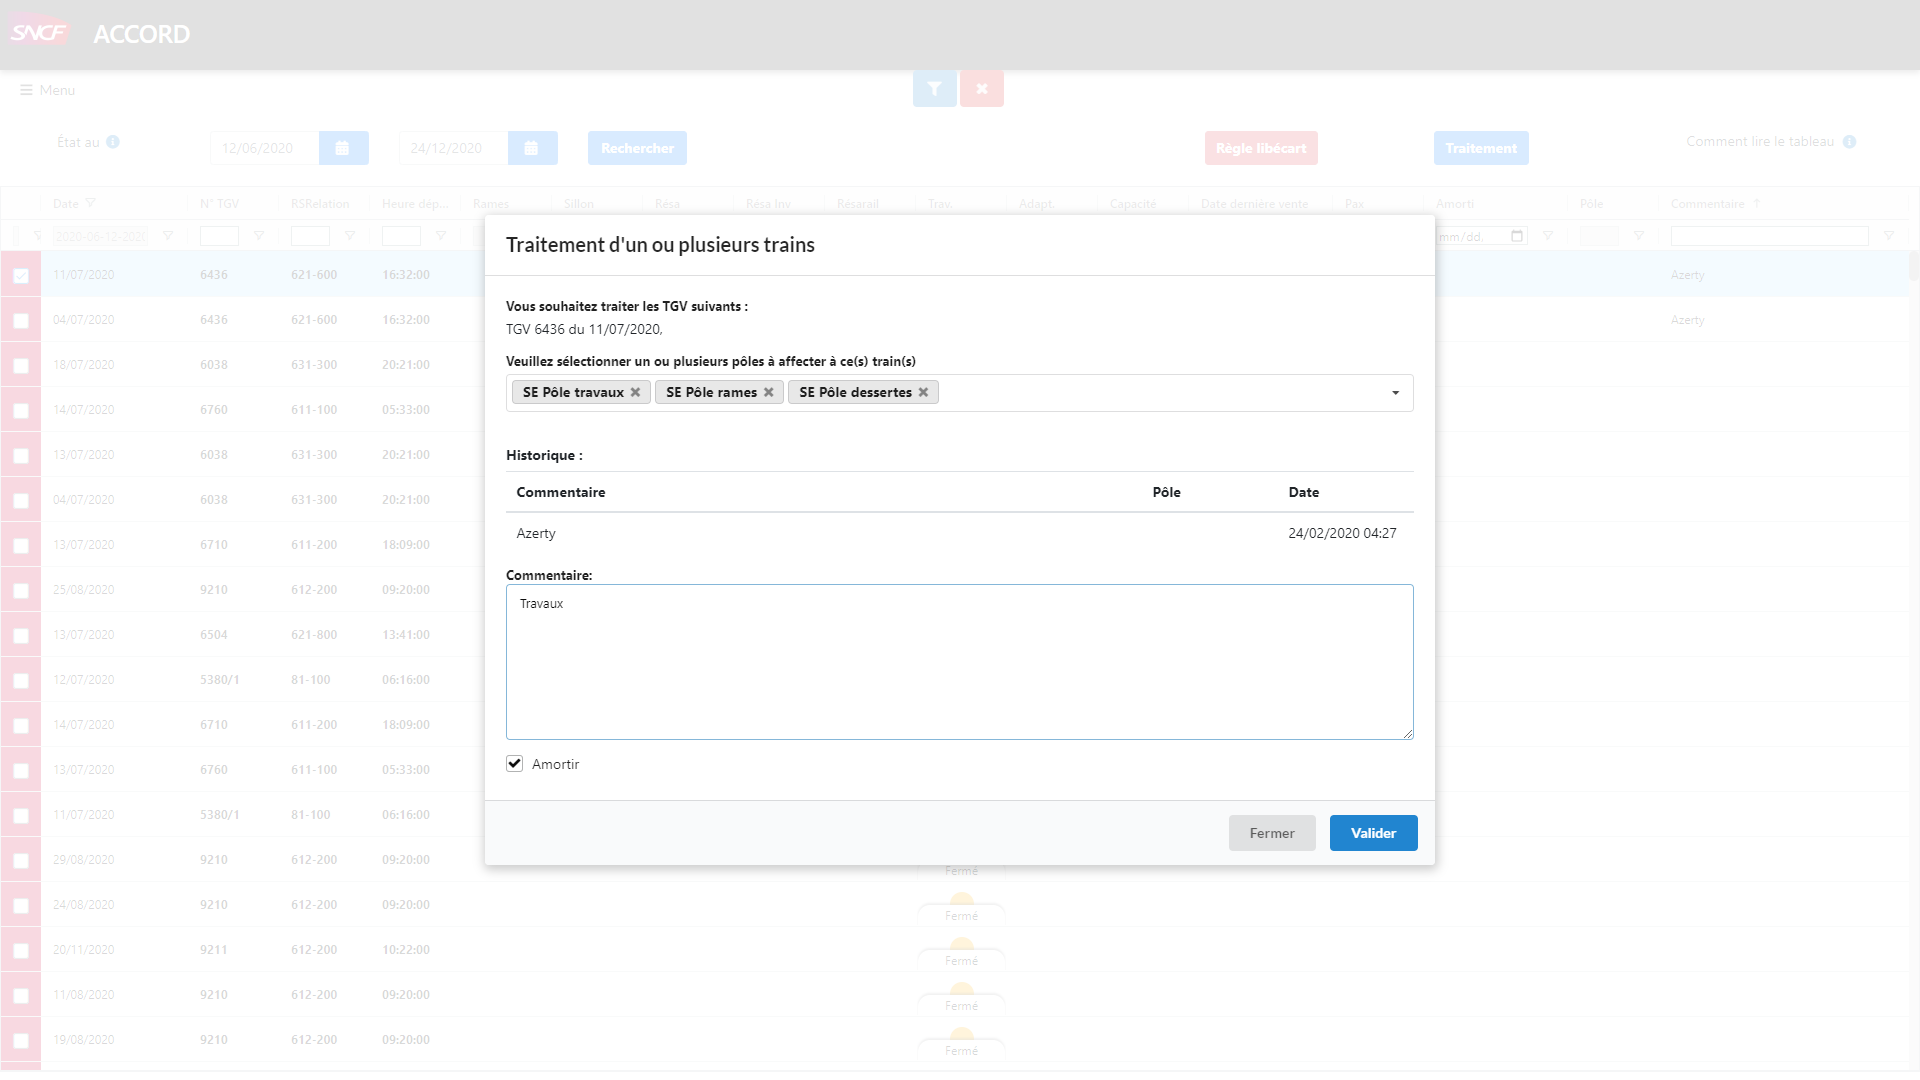
\includegraphics[width=1\linewidth]{img/sycomores_commentaire.png}
    \caption{Page de traitement de trains : commentaire, assignation de pôles et date d'amorti}
  \end{figure}

Enfin, j'ai créé l'écran présentant les mises à jour de données et l'état des traitements automatisés. Il permet aux utilisateurs de connaître la date de mise à jour de chacune des sources de données \sncf, ainsi que si le traitement automatique s'est déroulé sans rencontrer de problèmes.


  \begin{figure}[H]
    \centering
    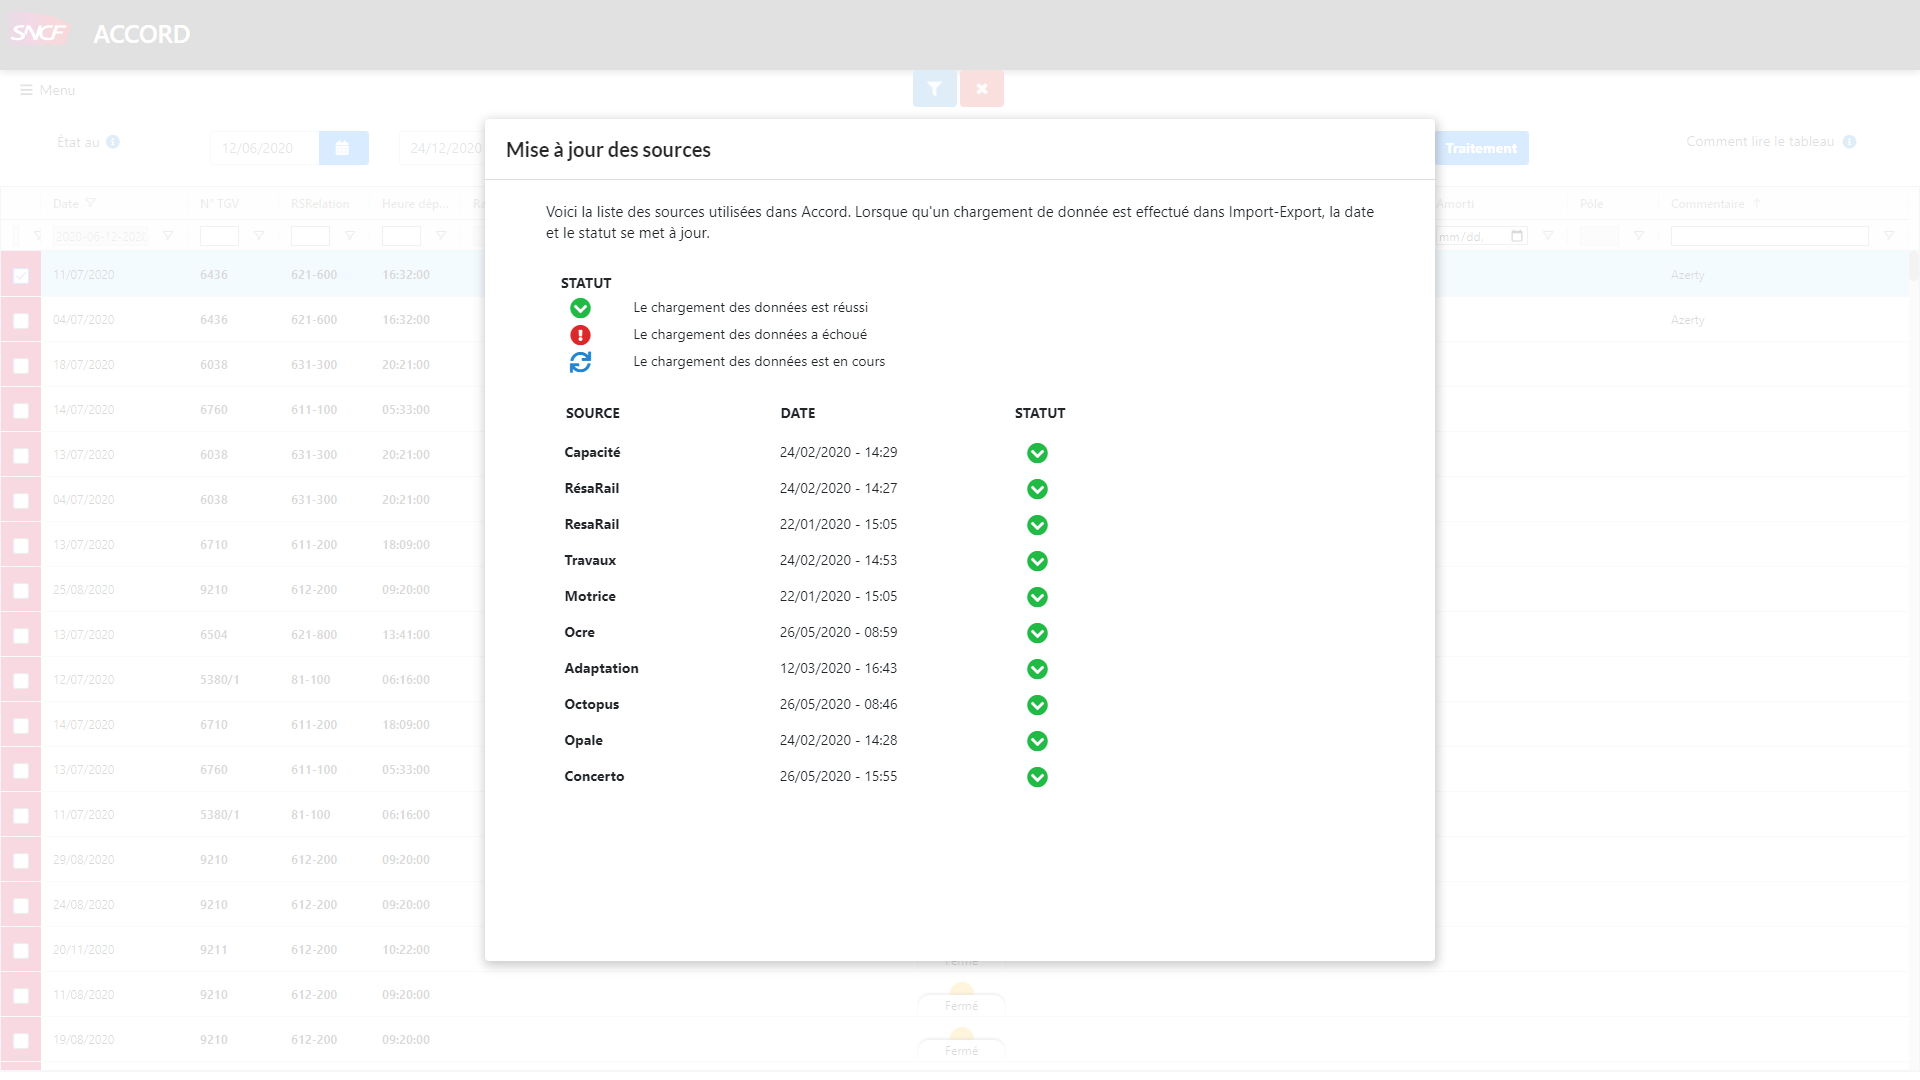
\includegraphics[width=1\linewidth]{img/sycomores_traitements.png}
    \caption{Écran de suivi des traitements et des dates de mises à jour des sources de données}
  \end{figure}

\newpage
\subsection{Le \textit{back-end}}

Nous avons fait le choix d'utiliser un \gls{back-end} sans serveur, en utilisant le service de calcul distribué d'\gls{aws}. Nous détaillerons ce point dans la partie suivante.

Ce projet était en collaboration avec l'équipe \ds, qui a peu l'habitude de travailler avec une interface web et de communiquer avec d'autres services. En effet, leur travail se concentre d'habitude sur de l'analyse de données.
Il fallait donc trouver une solution simple à appréhender pour eux.

En déléguant la gestion de serveur à \gls{aws}, les équipes n'avaient plus qu'à se focaliser sur la création d'algorithmes. Cela simplifie la tâche aux \ds, et fait également gagner du temps aux développeurs, puisqu'ils n'ont alors plus besoin de se soucier de la mise en place et la gestion des serveurs.

Le choix du langage de programmation a suivi la même logique. Les \ds avaient déjà l'habitude d'utiliser Python pour leurs algorithmes, qui reste une référence en traitement de données. C'est un langage assez simple à prendre en main, il ne posait donc pas de souci aux développeurs non plus.
Python souffre cependant d'un problème de rapidité d'exécution, ce qui peut parfois poser un problème. Dans notre cas, ce n'était pas un souci, puisque nous n'avions pas de traitement de données en temps réel à faire.

J'ai développé les fonctionnalités de la partie précédente côté serveur, à savoir la récupération des informations de mises à jour des sources de données, la gestion des règles lib-écarts, et la récupération des pôles d'affectation et des commentaires.

Le tâche la plus conséquente a été l'implémentation des fonctions liées aux données des trains : la récupération par blocs, les tris, les filtres, etc.
J'ai encore une fois travaillé sur cette partie en binôme avec Anthony \textsc{Mercadal}.

Enfin, j'ai mis en place le système d'authentification de l'application. L'emphase était mise sur les fonctionnalités métiers dont le client avait besoin, mais une page de connexion sécurisée était évidemment nécessaire.
J'ai décidé d'utiliser une authentification basée sur un \textit{JSON Web Token}, une solution standard du web qui a fait ses preuves.

  \begin{figure}[H]
    \centering
    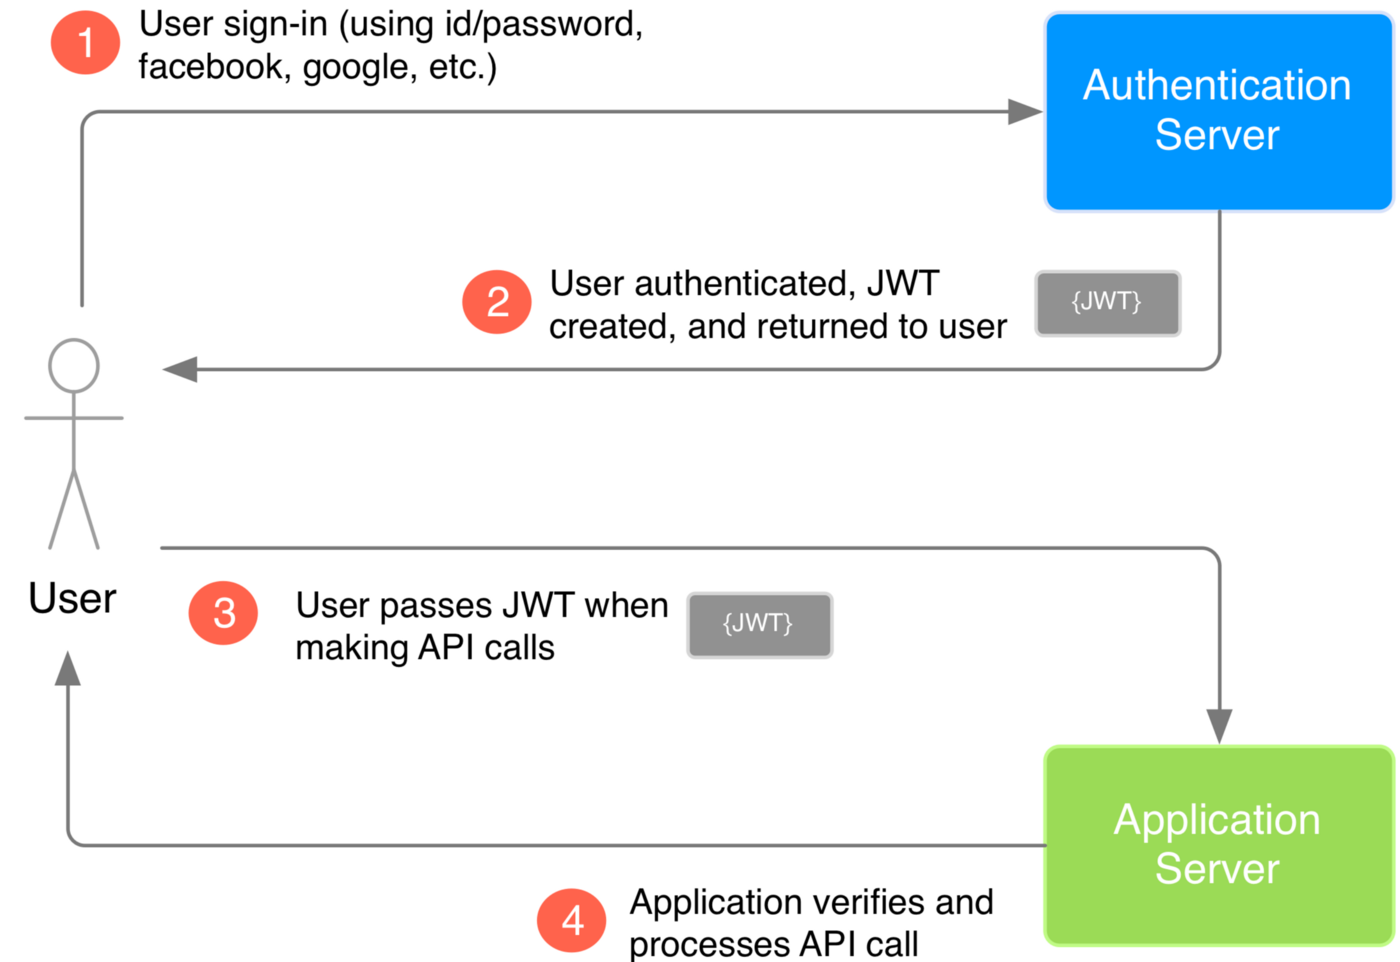
\includegraphics[width=1\linewidth]{img/jwt.png}
    \caption{Exemple classique d'utilisation d'un \textit{JSON Web Token} pour l'authentification}
  \end{figure}

Le principe est le suivant :

\newcommand{\user}{\textbf{utilisateur}\xspace}
\newcommand{\server}{\textbf{serveur}\xspace}

\begin{itemize}
    \item L'\user envoie son identifiant et mot de passe au \server
    \item Le \server créer un jeton d'authentification contenant des généralement des informations comme :
    \begin{itemize}
        \item La date et heure d'expiration du jeton
        \item L'identifiant de l'utilisateur
        \item N'importe quelle information utile (en gardant en tête que n'importe qui pourra lire cette information)
    \end{itemize}
    \item Le \server signe le jeton à l'aide d'un algorithme de chiffrement et d'une clé secrète
    \item Le \server envoie le jeton a l'\user
    \item L'\user connecté joindra son jeton à chaque requête au \server
    \item Le \server vérifie qu'il a bien créé le jeton grâce à la signature, dont il est le seul à connaître la clé secrète
    \item Si la signature est correcte, et que le jeton n'a pas expiré, le \server envoie la réponse à la requête de l'\user
\end{itemize}


% get poles (recupere liste des poles)
% put sycomores (insere un commentaire / met a jour)
% permissions (verifie le token jwt de la personne)
% put libecart (travail avec anthony: insertion de regle libecart)
% traitement (recupere la liste des batch AWS)
% sycomore (get les trains avec anthony)


% Outil avec SED qui permet de recuperer les nouvelles regles lib ecart depuis leur excel tout nul

\newpage
\subsection{\textsc{AWS}: l'infrastructure \textit{cloud}}

% S3 Buckets, Lambdas, API Gateway, Cloudfront.
% Batch

\tnp ne possède pas de système d'information interne, il n'était donc pas envisageable de stocker les données et gérer les serveurs d'applications dans nos locaux.
En effet, l'entreprise étant un cabinet de conseil, les employés n'ont besoin que de la suite d'outils de collaboration Office365 de Microsoft, comme Skype, Teams, Outlook, PowerPoint, etc.

Nous nous sommes donc dirigés vers une infrastructure \textit{cloud}. Les acteurs du marché proposent tous peu ou prou les mêmes services, il était alors difficile de les départager. Cependant, \tnp, via l'entité \textsc{TNP} Training, est partenaire \gls{aws}\cite{noauthor_tnp_nodate} et propose des formations et certifications \gls{aws}. Un expert certifié est d'ailleurs présent sur le site, nous nous sommes alors orientés vers ce service plutôt qu'un autre.

Pour notre mission, nous avions besoin des éléments suivants :

\begin{itemize}
    \item Une base de données afin de stocker les informations des différentes sources de données \sncf et des résultats des traitements
    \item Un service de calcul distribué pour exécuter nos algorithmes
    \item Un moyen de déclencher ces algorithmes et d'en récupérer le résultat, notamment pour que l'interface puisse afficher les données et envoyer des modifications
    \item Un service d'hébergement pour notre interface web afin de la rendre accessible depuis Internet
\end{itemize}

Amazon propose le service \textit{Relational Database Service (RDS)}\cite{noauthor_aws_nodate-2} pour l'hébergement d'une base de données. Plusieurs systèmes de gestion de base de données sont disponibles, nous avons choisi \emph{PostgreSQL}. C'est un système en \emph{source ouverte}, \emph{gratuit} et respectant à la lettre le standard \textsc{POSIX}\cite{noauthor_open_nodate}.

Une fois la base de données créée sur \gls{aws} on y accède comme n'importe quelle base de données hébergée sur un système d'information.

En ce qui concerne le service de \textit{cloud computing}, Amazon a le service Lambda\cite{noauthor_aws_nodate-1}. Il suffit de téléverser le code source sur Lambda en précisant le langage utilisé, et Amazon se charge de l'exécuter lorsque l'on demande. L'on peut même modifier le code source depuis l'interface \gls{aws}.

  \begin{figure}[H]
    \centering
    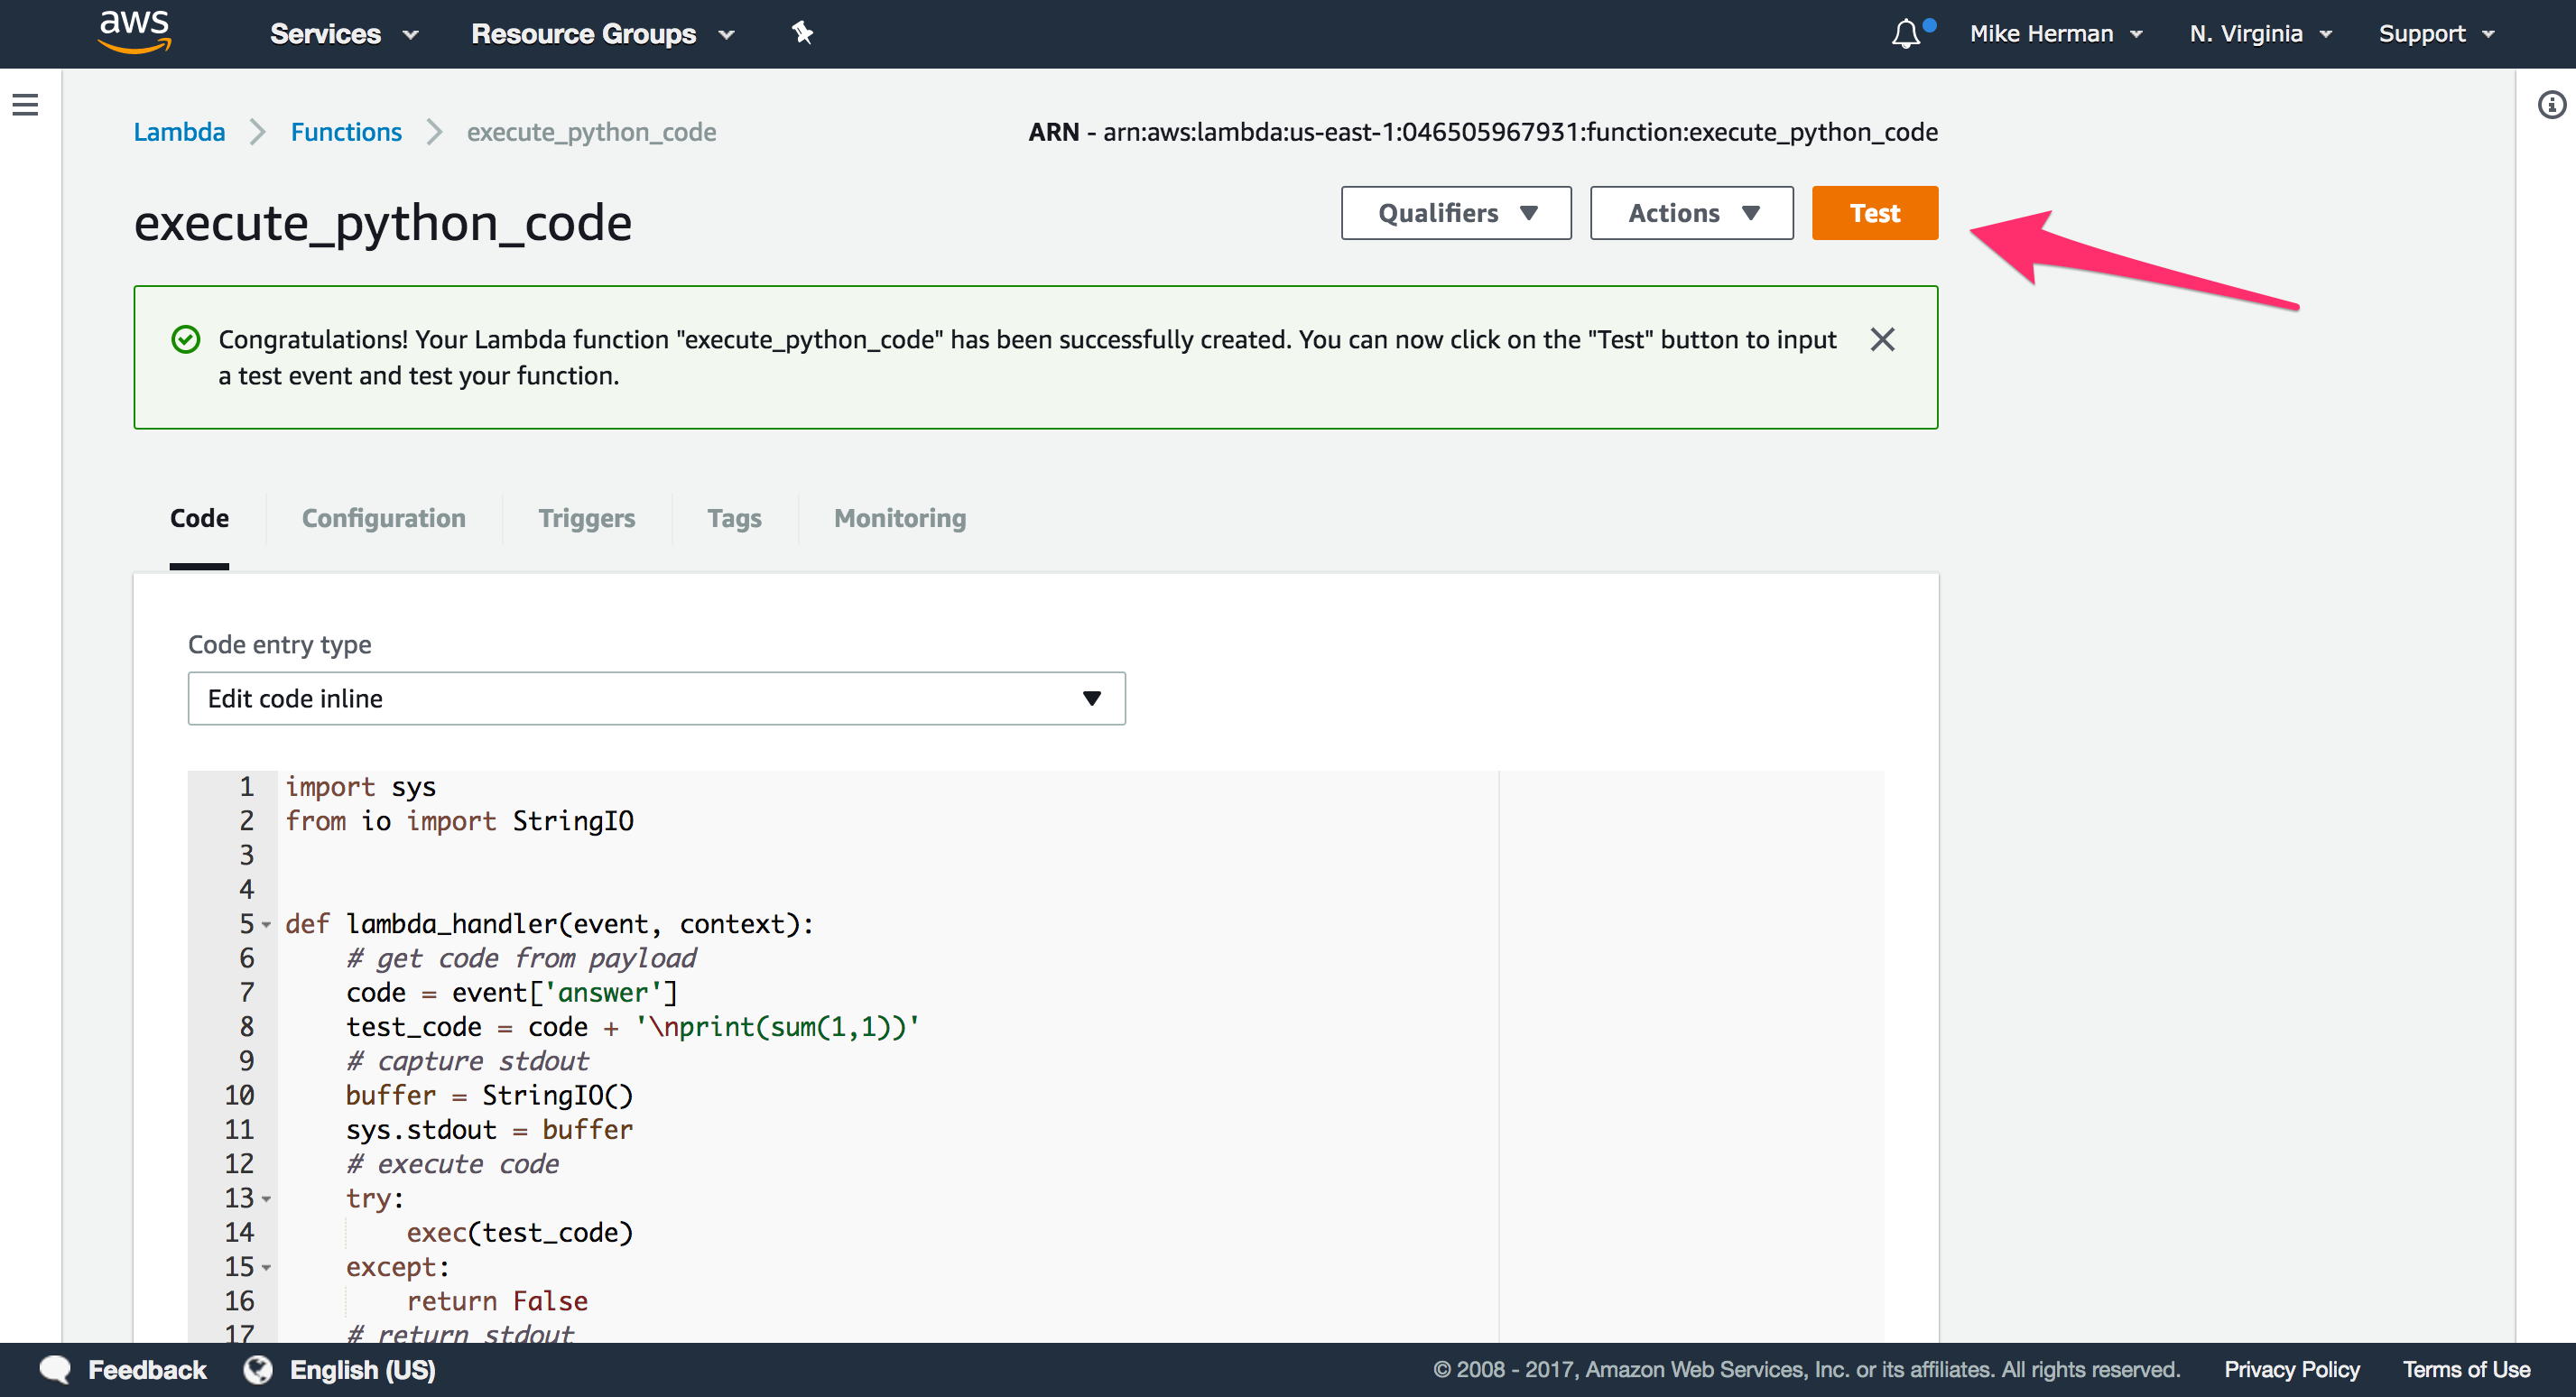
\includegraphics[width=1\linewidth]{img/aws_lambda_ui.png}
    \caption{Interface de gestion d'une fonction AWS Lambda : éditeur de code source en ligne et bouton d'exécution}
  \end{figure}

Afin d'héberger notre application web, nous nous sommes servis de Amazon S3. Il s'agit d'un service de stockage de fichiers, mais il peut être utilisé pour stocker et exposer un site.

Enfin,
API Gateway\cite{noauthor_conception_nodate-1}
nous a permis de faire le lien entre notre interface web et les algorithmes hébergés sur \gls{aws} Lambda.
En effet, ce service permet entre autres de déclencher les fonctions Lambda et de renvoyer le résultat en sortie. Il existe plusieurs manières de communiquer avec ce service, nous avons choisi de le faire via une
\gls{api}\footnote{\glsdesc{api}.}
\gls{rest}\footnote{\glsdesc{rest}.}
utilisant le protocole \textsc{HTTP}.

Depuis plusieurs années, il s'agit de la méthode de communication entre la partie \gls{front-end} et \gls{back-end} la plus répandue. Elle permet de manipuler des données via leurs représentations textuelles à travers un ensemble d'opérations uniformes, aussi bien au sein d'un projet que sur le web en général. En effet, les développeurs tendent à tous utiliser les mêmes conventions de nommage et d'accès aux ressources.

  \begin{figure}[H]
    \centering
    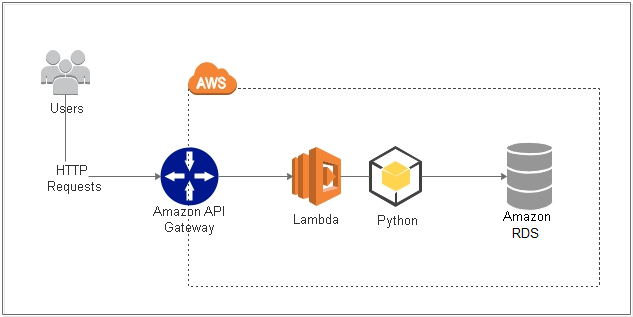
\includegraphics[width=1\linewidth]{img/aws_api_gateway.png}
    \caption{Schéma d'une requête HTTP depuis l'interface web vers l'API REST hébergée sur AWS}
  \end{figure}

Cela permet une lecture plus simple et rapide des \gls{api}. Chacun nomme les choses de la même manière, et sait intuitivement comment y accéder à force d'utiliser cette représentation.

\newpage
\subsection{Outils de déploiement de la solution}

% Bitbucket Pipelines via Serverless pour les lambdas et normal pour S3.

Ma mission consistait également à mettre en place des outils \gls{devops} pour faciliter le déploiement des services et le travail des développeurs.

Nous hébergeons notre code source sur Bitbucket\cite{noauthor_bitbucket_nodate}, qui vient avec la suite Atlassian dont nous parlerons ensuite. Il s'agit d'un serveur git en ligne permettant le stockage et le
\textit{versionning}\footnote{\og Gestion des versions \fg en français. Permet de gérer un ensemble de versions des fichiers. Surtout utilisé dans la gestion de code source dans les projets informatiques.}
de code source.

Bitbucket intègre également une chaîne de traitement,
\textit{Bitbucket Pipelines}\cite{noauthor_bitbucket_nodate-1}
. Grâce à cela, nous pouvons exécuter automatiquement des traitements en réponse à des événements. Par exemple, il est possible d'envoyer des fichiers sur Amazon S3 à chaque fois qu'un développeur publie son code.

C'est ce que nous avons mis en place pour le code source de l'interface web et des fonctions destinées à AWS Lambda.
Ainsi, à chaque mise à jour du code source de l'interface web Angular, \textit{Bitbucket Pipelines} construit le projet grâce aux outils d'Angular puis remplace les fichiers actuellement hébergés sur Amazon S3 avec les nouveaux.

Les développeurs ont alors en permanence un projet à jour, accessible depuis n'importe où.
Cela leur permet de vérifier très rapidement que tout fonctionne correctement, mais également de montrer les avancées aux managers. L'on peut également se servir de cela comme point de comparaison : comme le site est toujours à jour, on remarque rapidement si nos modifications ont changé quelque chose qu'elles ne devaient pas.

En parallèle de cette première \textit{pipeline}, une seconde a été créée pour publier les modifications sur un autre Amazon S3, celui servant pour la recette fonctionnelle du client.

En effet, il n'est pas souhaitable que l'interface sur laquelle le client effectue ses tests soit aussi instable et si souvent mise à jour. Nous avons donc mis en place une seconde \textit{pipeline} -- déclenchée manuellement cette fois-ci -- qui construit le projet et envoie les fichiers vers le S3 de recette fonctionnelle.
Elle est déclenchée à chaque fois que l'on estime avoir un projet stable.

Nous aurions pu suivre la même méthode pour le déploiement automatique des fonctions destinées à AWS Lambda. On aurait alors dû, pour chaque fonction, télécharger les dépendances, mettre le code source dans une archive et téléverser cette archive sur AWS Lambda.\\
Ensuite, pour chaque fonction, il aurait fallu créé un déclencheur dans API Gateway afin de pouvoir lancer l'exécution et récupérer le résultat depuis un service externe.
Cependant, il existe un outil qui simplifie grandement ce travail : \textit{Serverless}\cite{noauthor_serverless_nodate}.

\textit{Serverless} automatise cette procédure en publiant chaque fonction dans AWS Lambda et en créant le déclencheur associé sur AWS API Gateway tout seul.

Ainsi, tout comme l'interface web, le \gls{back-end} est toujours à jour par rapport au code source. Chaque modification est répercutée dans les minutes qui suivent la publication du code, et les développeurs peuvent immédiatement voir le fruit de leur travail.

Ces outils simplifient grandement le déploiement et la mise en production des solutions développées. De plus, ils permettent aux développeurs d'avoir plus conscience de ce qu'il se passe côté opérations et ainsi de mieux comprendre leur environnement de travail.

\newpage
\subsection{Organisation, gestion et suivi des tâches}

La \df suit un processus de développement \gls{scrum}. Un des outils de référence dans la gestion de projets est Jira -- compris avec Bitbucket et Confluence dans la suite Atlassian --, qui intègre cette méthode de travail.

Jira permet dans un premier temps de remplir le carnet de produit (\textit{product backlog}) avec toutes les tâches fonctionnelles à réaliser pour le projet.


  \begin{figure}[H]
    \centering
    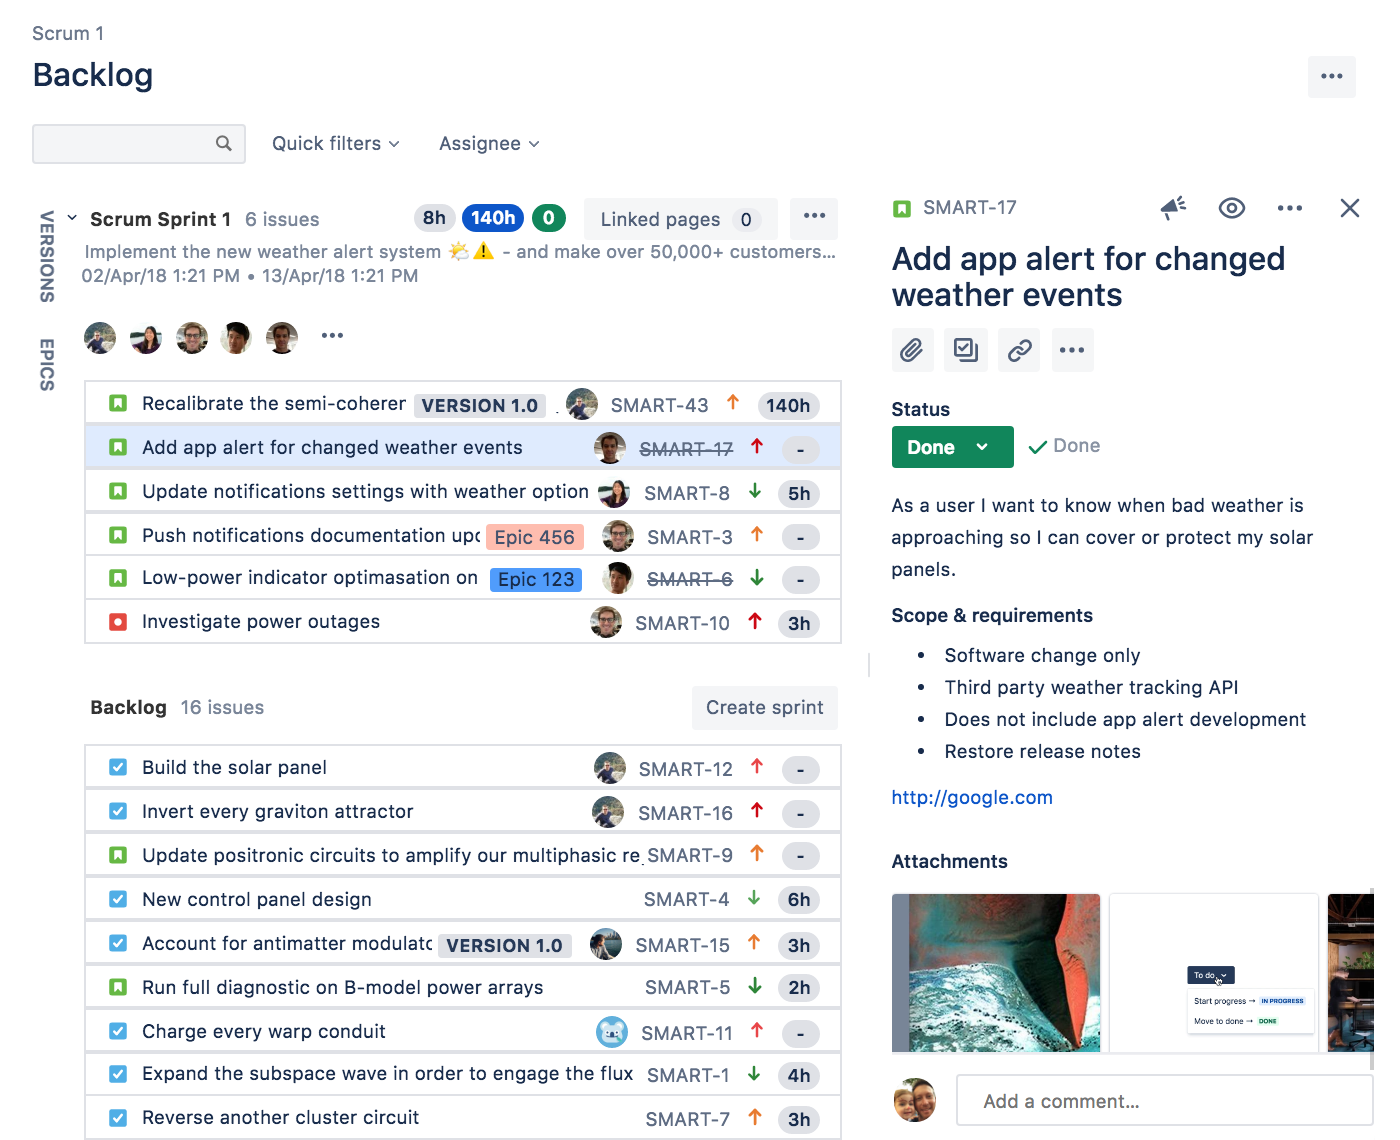
\includegraphics[width=1\linewidth]{img/jira_Scrum_backlog.png}
    \caption{Carnet de produit sur Jira}
  \end{figure}

Une fois le carnet rempli, les équipes peuvent se réunir en début de \textit{sprint} pour planifier et décider des tâches qui seront effectuées durant la période en remplissant le carnet de sprint (\textit{sprint backlog}). Chaque tâche peut être assignée à une personne de l'équipe et est forcément rattachée à un responsable. On peut également lui attribuer des points en fonction de sa difficulté.

Jira propose alors une vue sous forme de tableau pour suivre facilement l'évolution de chacune des tâches du \textit{sprint}.

  \begin{figure}[H]
    \centering
    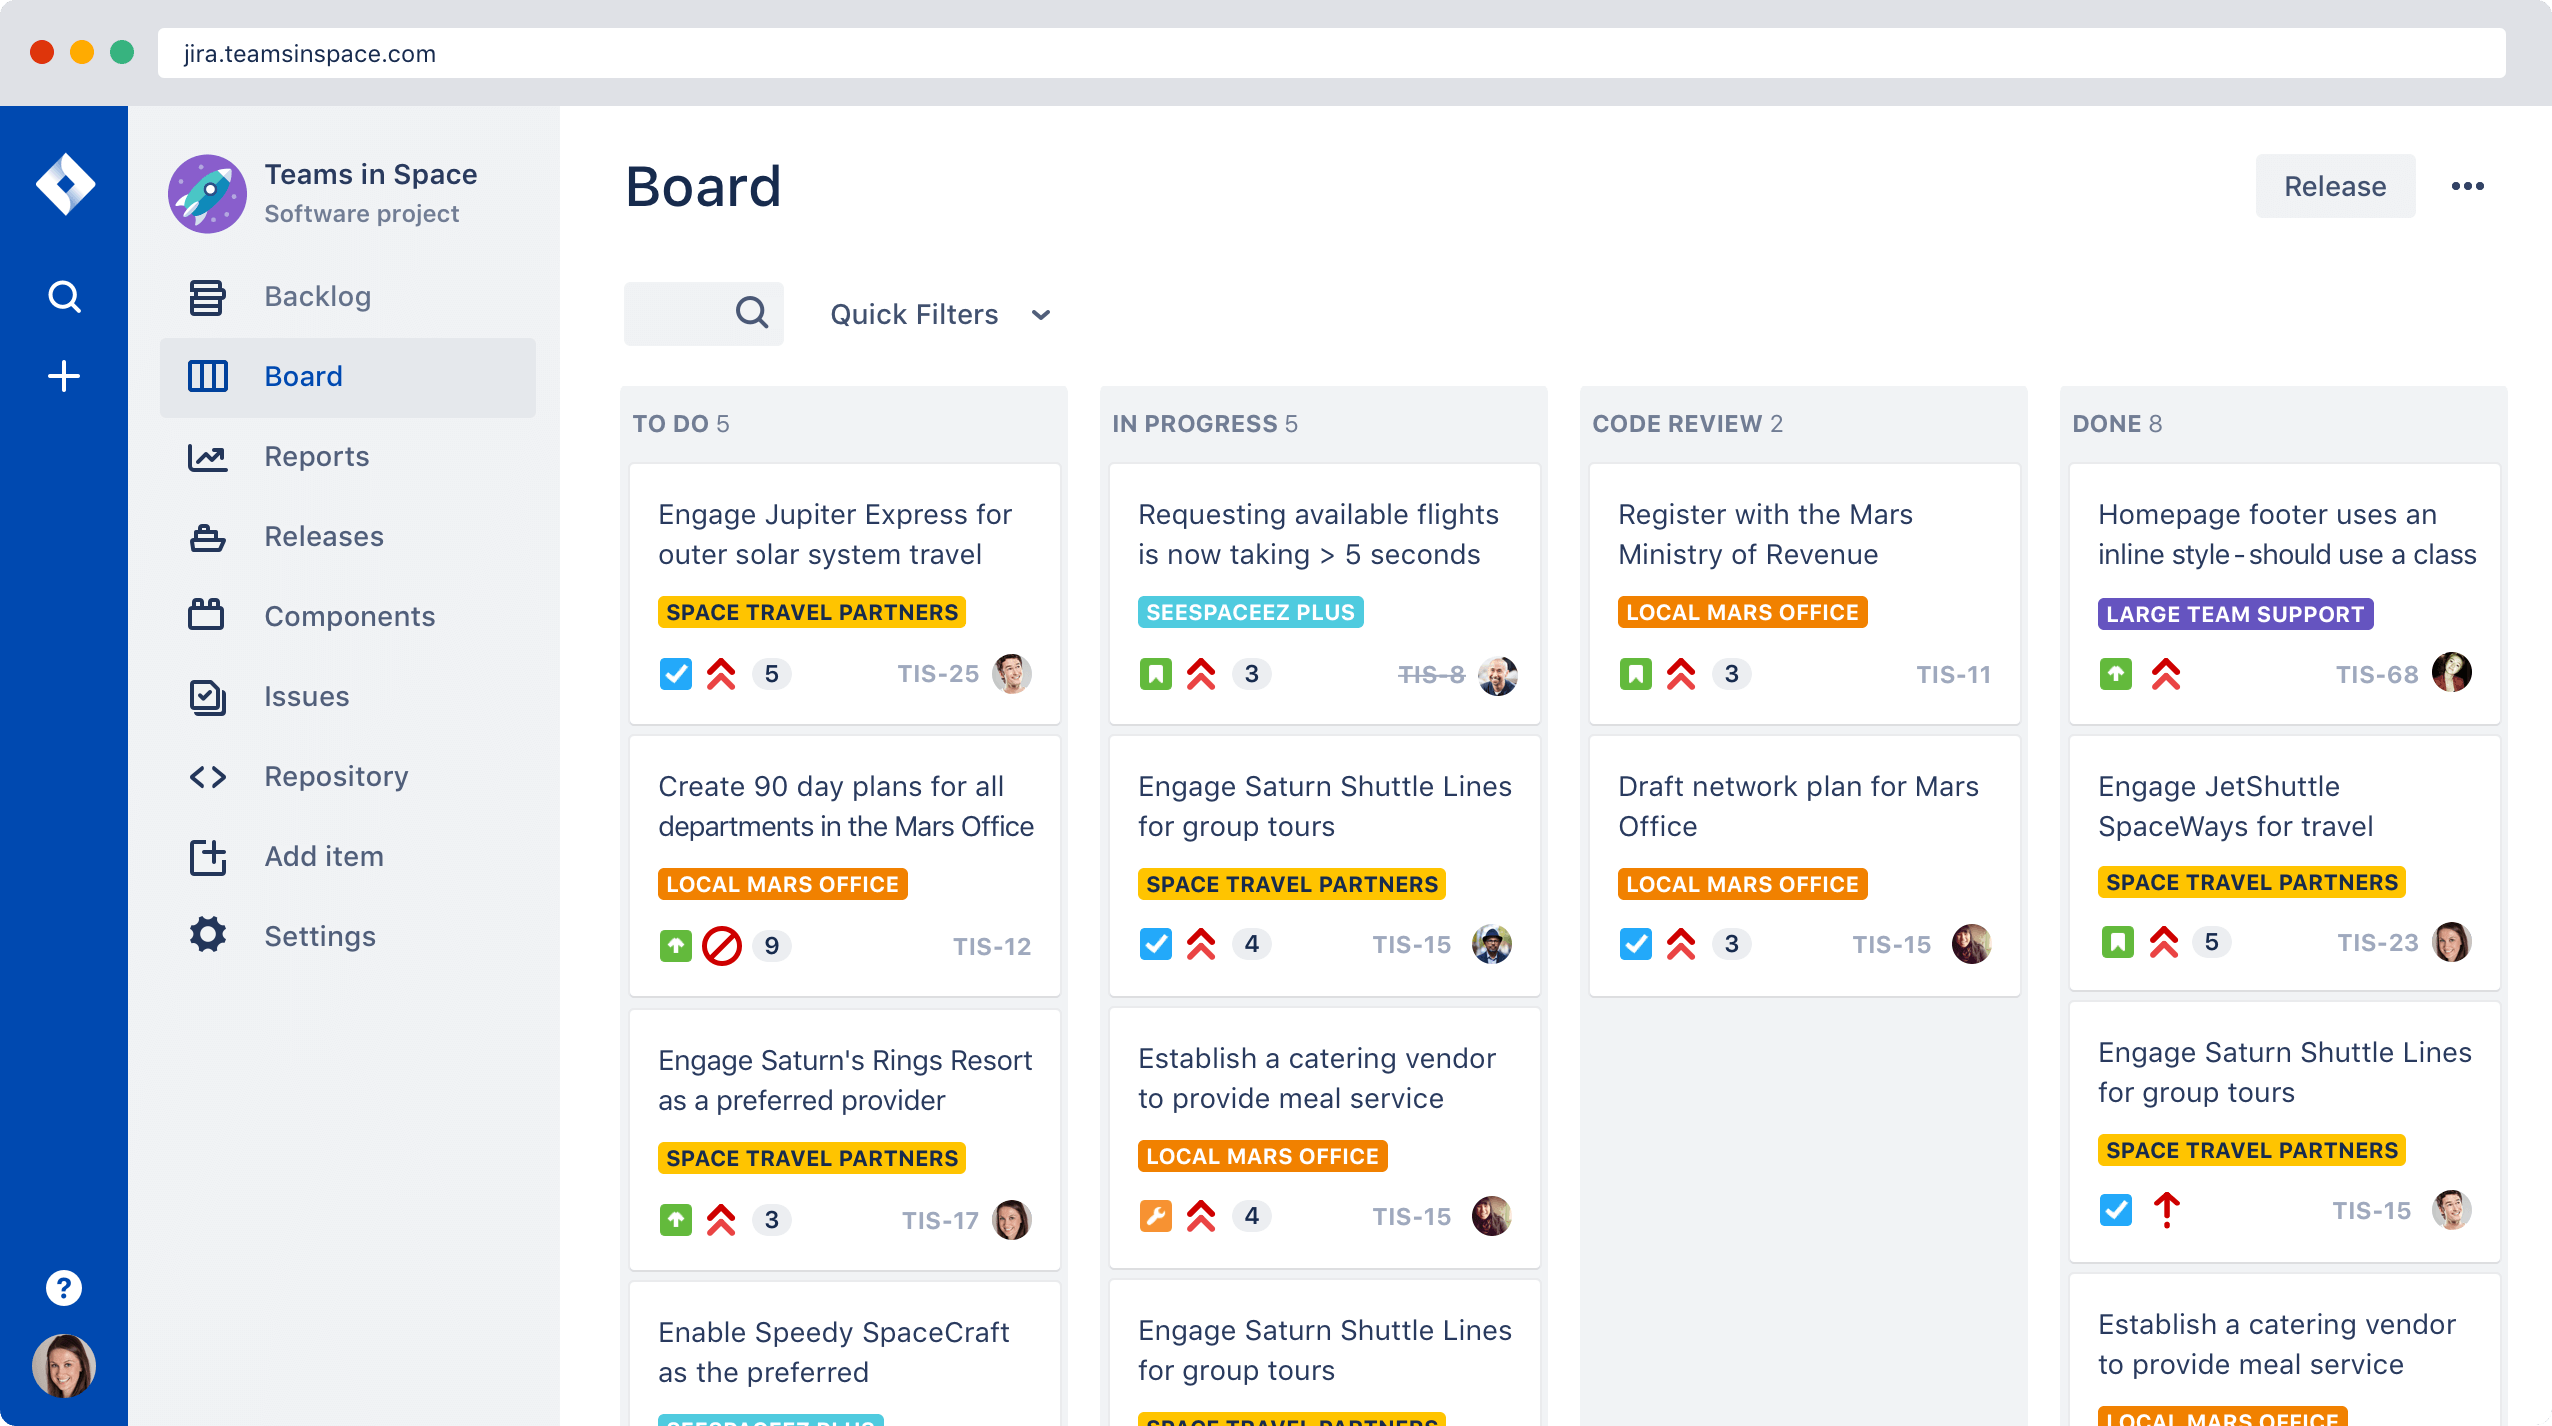
\includegraphics[width=1\linewidth]{img/jira_board.png}
    \caption{Tableau des tâches du \textit{sprint} en cours sur Jira}
  \end{figure}
  
Une fois le \textit{sprint} terminé, Jira aide lors de la revue de sprint en fournissant des statistiques et graphiques sur la période.

  \begin{figure}[H]
    \centering
    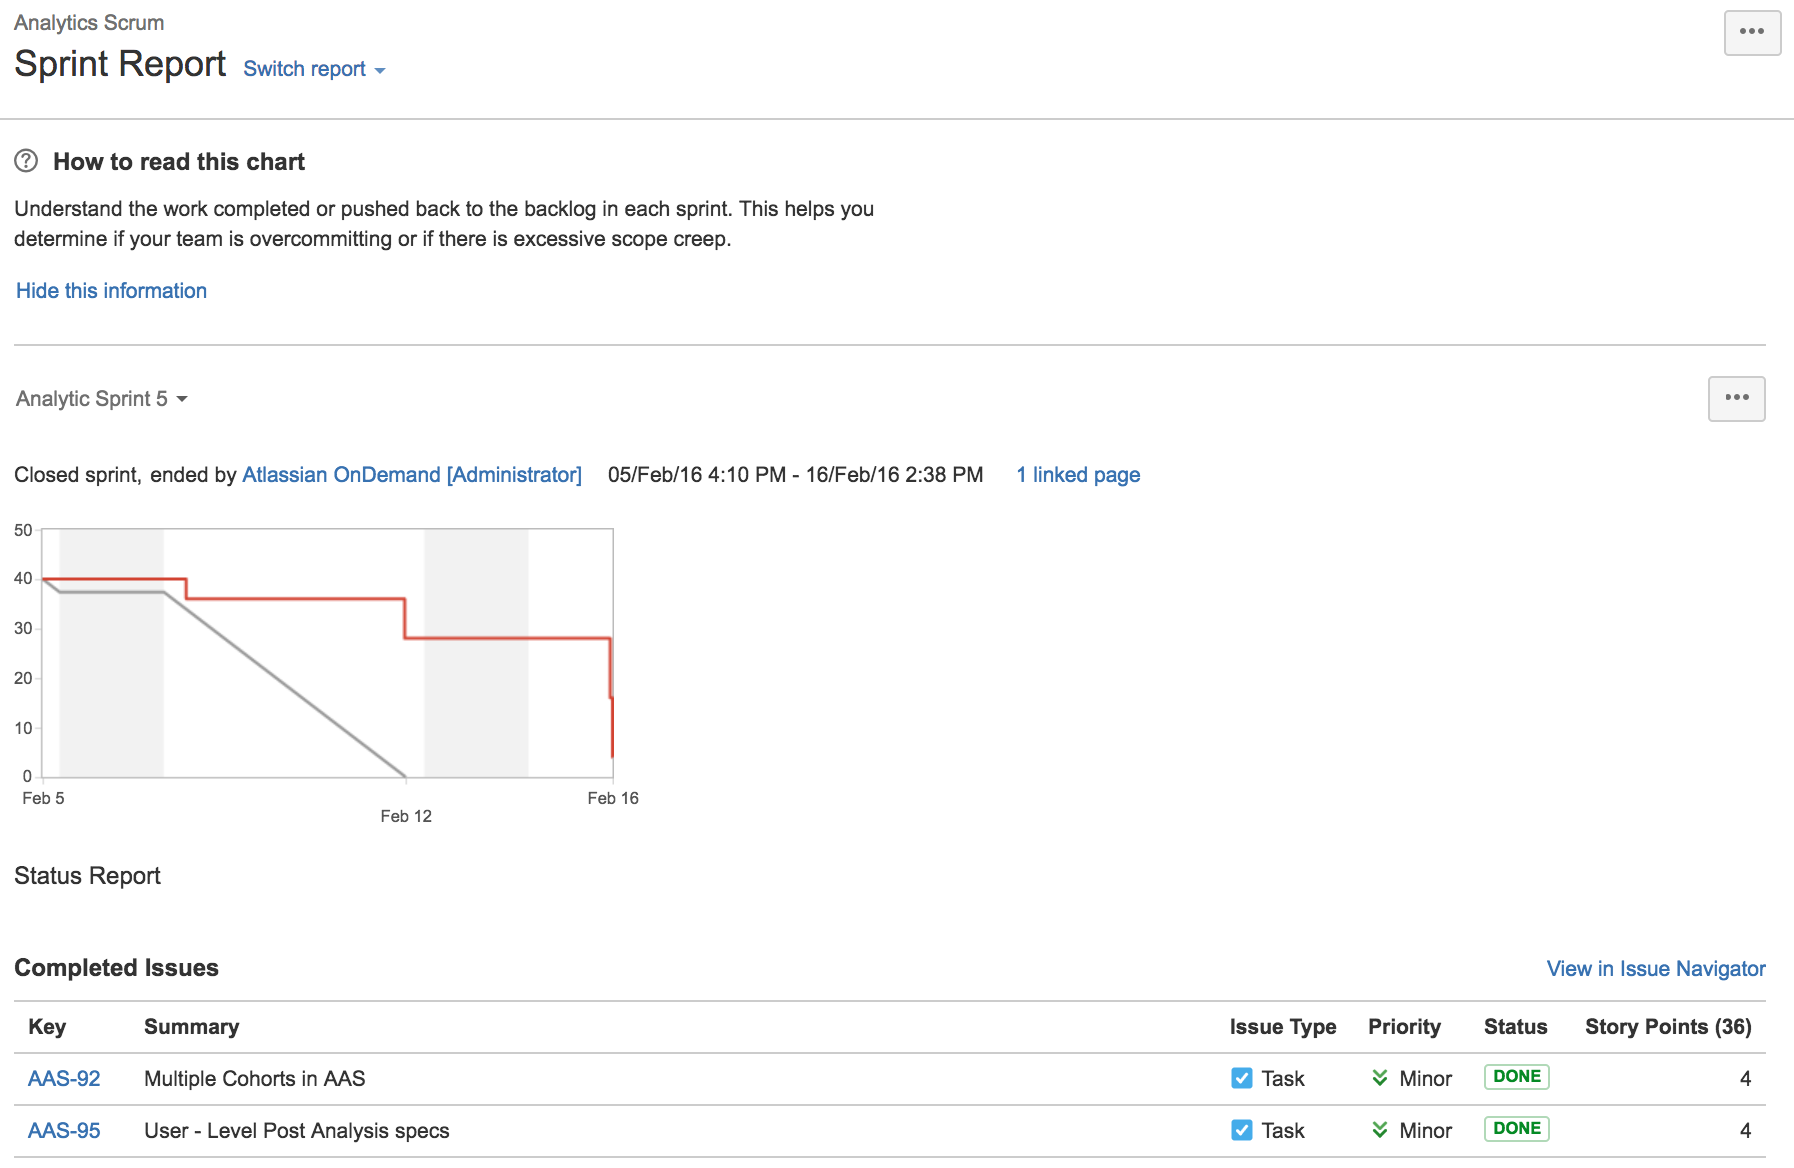
\includegraphics[width=1\linewidth]{img/jira-sprint-report.png}
    \caption{Rapport de fin de \textit{sprint} généré par Jira}
  \end{figure}
  
L'outil peut également servir pour la recette fonctionnelle, puisqu'une fonctionnalité de \textit{bug tracking} existe.

Enfin, la suite Atlassian vient avec Confluence, un outil de documentation et partage de documents. Il nous est utile pour garder une trace des informations importantes et partager des connaissances entre développeurs. Cela nous a par exemple été d'une grande aide pour centraliser et synthétiser toutes les informations que nous avions comprises sur les données de la \sncf.

  \begin{figure}[H]
    \centering
    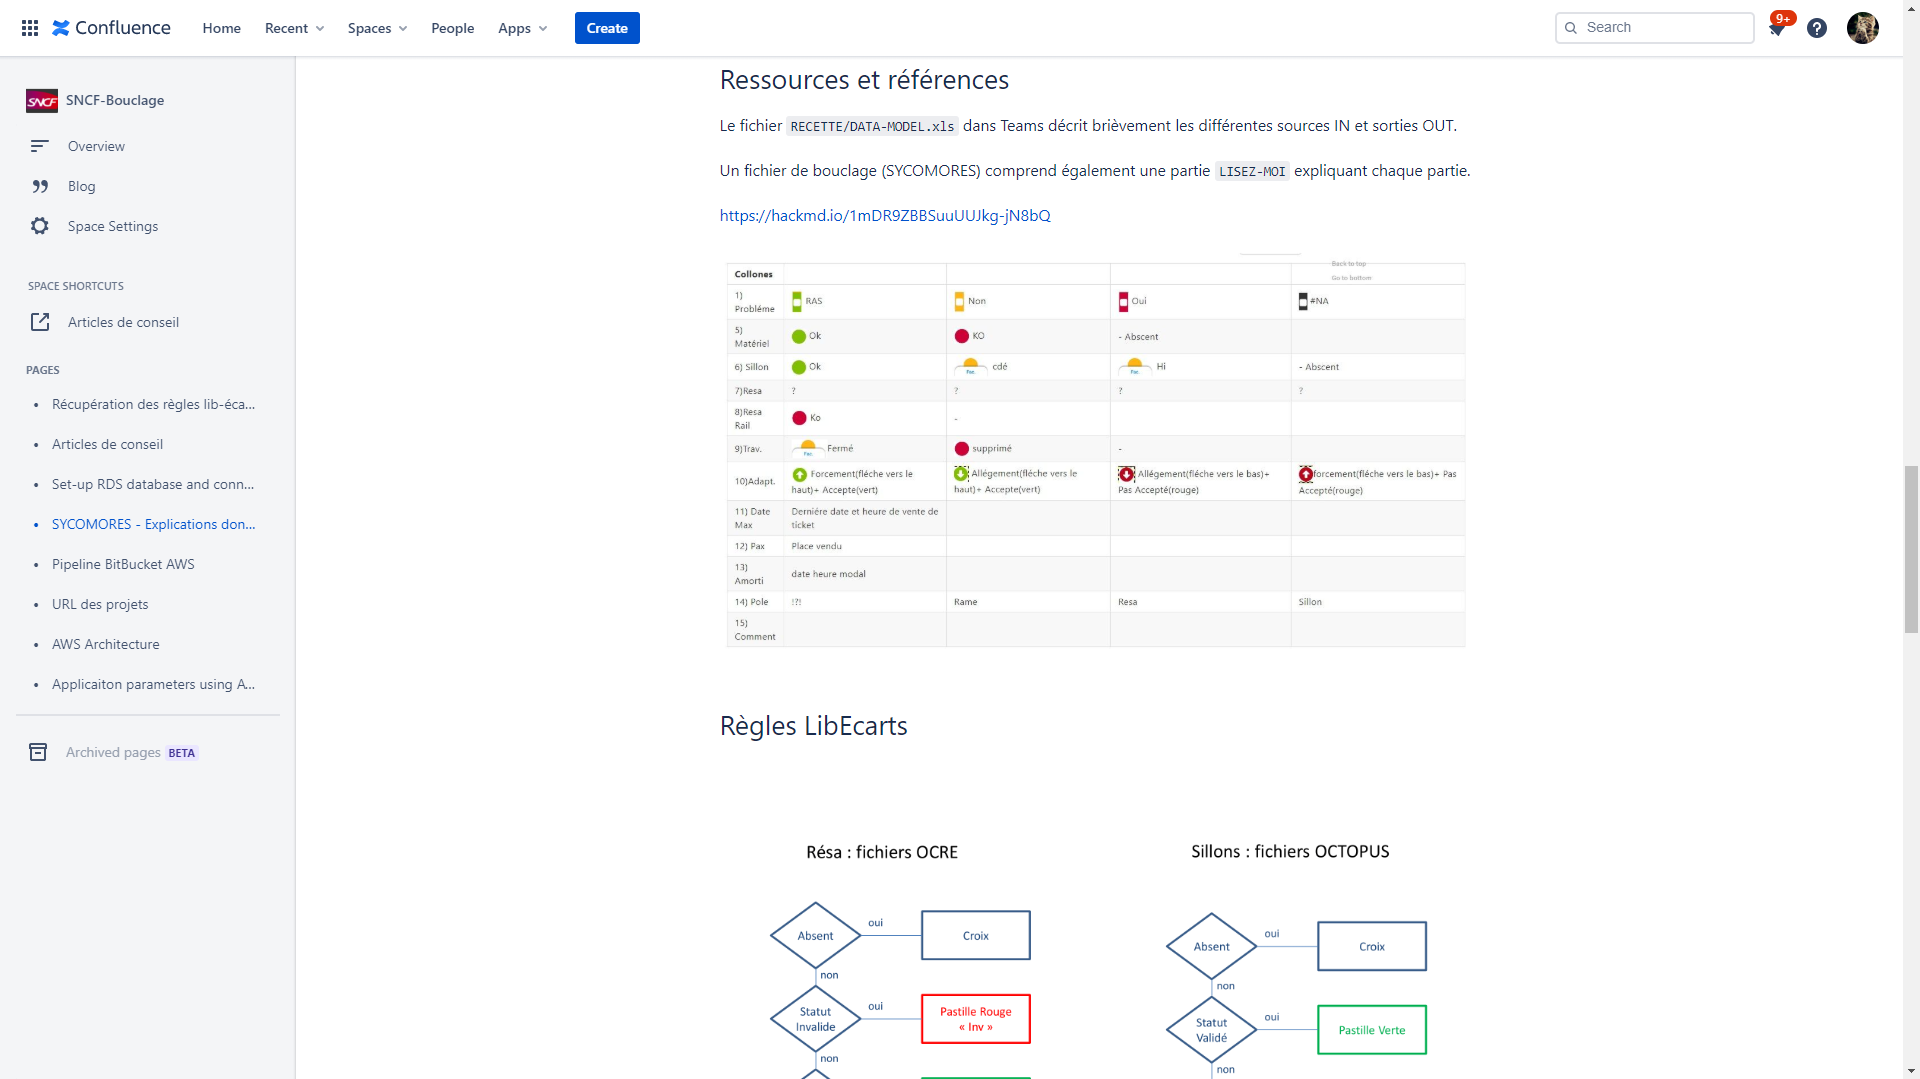
\includegraphics[width=1\linewidth]{img/confluence_sycomores_explications.png}
    \caption{Exemple de page Confluence : document de centralisation des clés de compréhension du projet bouclage de production}
  \end{figure}